\documentclass[twoside]{book}

% Packages required by doxygen
\usepackage{fixltx2e}
\usepackage{calc}
\usepackage{doxygen}
\usepackage[export]{adjustbox} % also loads graphicx
\usepackage{graphicx}
\usepackage[utf8]{inputenc}
\usepackage{makeidx}
\usepackage{multicol}
\usepackage{multirow}
\PassOptionsToPackage{warn}{textcomp}
\usepackage{textcomp}
\usepackage[nointegrals]{wasysym}
\usepackage[table]{xcolor}

% Font selection
\usepackage[T1]{fontenc}
\usepackage[scaled=.90]{helvet}
\usepackage{courier}
\usepackage{amssymb}
\usepackage{sectsty}
\renewcommand{\familydefault}{\sfdefault}
\allsectionsfont{%
  \fontseries{bc}\selectfont%
  \color{darkgray}%
}
\renewcommand{\DoxyLabelFont}{%
  \fontseries{bc}\selectfont%
  \color{darkgray}%
}
\newcommand{\+}{\discretionary{\mbox{\scriptsize$\hookleftarrow$}}{}{}}

% Page & text layout
\usepackage{geometry}
\geometry{%
  a4paper,%
  top=2.5cm,%
  bottom=2.5cm,%
  left=2.5cm,%
  right=2.5cm%
}
\tolerance=750
\hfuzz=15pt
\hbadness=750
\setlength{\emergencystretch}{15pt}
\setlength{\parindent}{0cm}
\setlength{\parskip}{3ex plus 2ex minus 2ex}
\makeatletter
\renewcommand{\paragraph}{%
  \@startsection{paragraph}{4}{0ex}{-1.0ex}{1.0ex}{%
    \normalfont\normalsize\bfseries\SS@parafont%
  }%
}
\renewcommand{\subparagraph}{%
  \@startsection{subparagraph}{5}{0ex}{-1.0ex}{1.0ex}{%
    \normalfont\normalsize\bfseries\SS@subparafont%
  }%
}
\makeatother

% Headers & footers
\usepackage{fancyhdr}
\pagestyle{fancyplain}
\fancyhead[LE]{\fancyplain{}{\bfseries\thepage}}
\fancyhead[CE]{\fancyplain{}{}}
\fancyhead[RE]{\fancyplain{}{\bfseries\leftmark}}
\fancyhead[LO]{\fancyplain{}{\bfseries\rightmark}}
\fancyhead[CO]{\fancyplain{}{}}
\fancyhead[RO]{\fancyplain{}{\bfseries\thepage}}
\fancyfoot[LE]{\fancyplain{}{}}
\fancyfoot[CE]{\fancyplain{}{}}
\fancyfoot[RE]{\fancyplain{}{\bfseries\scriptsize Generated by Doxygen }}
\fancyfoot[LO]{\fancyplain{}{\bfseries\scriptsize Generated by Doxygen }}
\fancyfoot[CO]{\fancyplain{}{}}
\fancyfoot[RO]{\fancyplain{}{}}
\renewcommand{\footrulewidth}{0.4pt}
\renewcommand{\chaptermark}[1]{%
  \markboth{#1}{}%
}
\renewcommand{\sectionmark}[1]{%
  \markright{\thesection\ #1}%
}

% Indices & bibliography
\usepackage{natbib}
\usepackage[titles]{tocloft}
\setcounter{tocdepth}{3}
\setcounter{secnumdepth}{5}
\makeindex

% Hyperlinks (required, but should be loaded last)
\usepackage{ifpdf}
\ifpdf
  \usepackage[pdftex,pagebackref=true]{hyperref}
\else
  \usepackage[ps2pdf,pagebackref=true]{hyperref}
\fi
\hypersetup{%
  colorlinks=true,%
  linkcolor=blue,%
  citecolor=blue,%
  unicode%
}

% Custom commands
\newcommand{\clearemptydoublepage}{%
  \newpage{\pagestyle{empty}\cleardoublepage}%
}

\usepackage{caption}
\captionsetup{labelsep=space,justification=centering,font={bf},singlelinecheck=off,skip=4pt,position=top}

%===== C O N T E N T S =====

\begin{document}

% Titlepage & ToC
\hypersetup{pageanchor=false,
             bookmarksnumbered=true,
             pdfencoding=unicode
            }
\pagenumbering{roman}
\begin{titlepage}
\vspace*{7cm}
\begin{center}%
{\Large C\+S354R Final Project \+: F\+PS Using Custom Open\+GL 3.3 Renderer \char`\"{}\+Larp\char`\"{} }\\
\vspace*{1cm}
{\large Generated by Doxygen 1.8.11}\\
\end{center}
\end{titlepage}
\clearemptydoublepage
\tableofcontents
\clearemptydoublepage
\pagenumbering{arabic}
\hypersetup{pageanchor=true}

%--- Begin generated contents ---
\chapter{Hierarchical Index}
\section{Class Hierarchy}
This inheritance list is sorted roughly, but not completely, alphabetically\+:\begin{DoxyCompactList}
\item \contentsline{section}{Camera}{\pageref{classCamera}}{}
\item \contentsline{section}{Larp\+:\+:Configuration\+Loader}{\pageref{classLarp_1_1ConfigurationLoader}}{}
\item enable\+\_\+shared\+\_\+from\+\_\+this\begin{DoxyCompactList}
\item \contentsline{section}{Larp\+:\+:Node}{\pageref{classLarp_1_1Node}}{}
\end{DoxyCompactList}
\item \contentsline{section}{Larp\+:\+:Entity}{\pageref{classLarp_1_1Entity}}{}
\item \contentsline{section}{Larp\+:\+:Mesh}{\pageref{classLarp_1_1Mesh}}{}
\item \contentsline{section}{Larp\+:\+:Model}{\pageref{classLarp_1_1Model}}{}
\item \contentsline{section}{Larp\+:\+:Scene\+Graph}{\pageref{classLarp_1_1SceneGraph}}{}
\item \contentsline{section}{Larp\+:\+:Shader}{\pageref{classLarp_1_1Shader}}{}
\item \contentsline{section}{Larp\+:\+:Texture}{\pageref{classLarp_1_1Texture}}{}
\item \contentsline{section}{Larp\+:\+:Vertex}{\pageref{structLarp_1_1Vertex}}{}
\end{DoxyCompactList}

\chapter{Class Index}
\section{Class List}
Here are the classes, structs, unions and interfaces with brief descriptions\+:\begin{DoxyCompactList}
\item\contentsline{section}{\hyperlink{classCamera}{Camera} }{\pageref{classCamera}}{}
\item\contentsline{section}{\hyperlink{classLarp_1_1ConfigurationLoader}{Larp\+::\+Configuration\+Loader} }{\pageref{classLarp_1_1ConfigurationLoader}}{}
\item\contentsline{section}{\hyperlink{classLarp_1_1Entity}{Larp\+::\+Entity} }{\pageref{classLarp_1_1Entity}}{}
\item\contentsline{section}{\hyperlink{classLarp_1_1Mesh}{Larp\+::\+Mesh} }{\pageref{classLarp_1_1Mesh}}{}
\item\contentsline{section}{\hyperlink{classLarp_1_1Model}{Larp\+::\+Model} }{\pageref{classLarp_1_1Model}}{}
\item\contentsline{section}{\hyperlink{classLarp_1_1Node}{Larp\+::\+Node} }{\pageref{classLarp_1_1Node}}{}
\item\contentsline{section}{\hyperlink{classLarp_1_1SceneGraph}{Larp\+::\+Scene\+Graph} }{\pageref{classLarp_1_1SceneGraph}}{}
\item\contentsline{section}{\hyperlink{classLarp_1_1Shader}{Larp\+::\+Shader} }{\pageref{classLarp_1_1Shader}}{}
\item\contentsline{section}{\hyperlink{classLarp_1_1Texture}{Larp\+::\+Texture} }{\pageref{classLarp_1_1Texture}}{}
\item\contentsline{section}{\hyperlink{structLarp_1_1Vertex}{Larp\+::\+Vertex} }{\pageref{structLarp_1_1Vertex}}{}
\end{DoxyCompactList}

\chapter{File Index}
\section{File List}
Here is a list of all files with brief descriptions\+:\begin{DoxyCompactList}
\item\contentsline{section}{src/\hyperlink{Camera_8cpp}{Camera.\+cpp} }{\pageref{Camera_8cpp}}{}
\item\contentsline{section}{src/\hyperlink{Camera_8hpp}{Camera.\+hpp} }{\pageref{Camera_8hpp}}{}
\item\contentsline{section}{src/\hyperlink{Entity_8cpp}{Entity.\+cpp} }{\pageref{Entity_8cpp}}{}
\item\contentsline{section}{src/\hyperlink{Entity_8hpp}{Entity.\+hpp} }{\pageref{Entity_8hpp}}{}
\item\contentsline{section}{src/\hyperlink{Error_8hpp}{Error.\+hpp} }{\pageref{Error_8hpp}}{}
\item\contentsline{section}{src/\hyperlink{Mesh_8cpp}{Mesh.\+cpp} }{\pageref{Mesh_8cpp}}{}
\item\contentsline{section}{src/\hyperlink{Mesh_8hpp}{Mesh.\+hpp} }{\pageref{Mesh_8hpp}}{}
\item\contentsline{section}{src/\hyperlink{Model_8cpp}{Model.\+cpp} }{\pageref{Model_8cpp}}{}
\item\contentsline{section}{src/\hyperlink{Model_8hpp}{Model.\+hpp} }{\pageref{Model_8hpp}}{}
\item\contentsline{section}{src/\hyperlink{Node_8cpp}{Node.\+cpp} }{\pageref{Node_8cpp}}{}
\item\contentsline{section}{src/\hyperlink{Node_8hpp}{Node.\+hpp} }{\pageref{Node_8hpp}}{}
\item\contentsline{section}{src/\hyperlink{RootNode_8hpp}{Root\+Node.\+hpp} }{\pageref{RootNode_8hpp}}{}
\item\contentsline{section}{src/\hyperlink{SceneGraph_8cpp}{Scene\+Graph.\+cpp} }{\pageref{SceneGraph_8cpp}}{}
\item\contentsline{section}{src/\hyperlink{SceneGraph_8hpp}{Scene\+Graph.\+hpp} }{\pageref{SceneGraph_8hpp}}{}
\item\contentsline{section}{src/\hyperlink{Shader_8cpp}{Shader.\+cpp} }{\pageref{Shader_8cpp}}{}
\item\contentsline{section}{src/\hyperlink{Shader_8hpp}{Shader.\+hpp} }{\pageref{Shader_8hpp}}{}
\item\contentsline{section}{src/\hyperlink{test_8cpp}{test.\+cpp} }{\pageref{test_8cpp}}{}
\end{DoxyCompactList}

\chapter{Class Documentation}
\hypertarget{classCamera}{\section{Camera Class Reference}
\label{classCamera}\index{Camera@{Camera}}
}


{\ttfamily \#include $<$Camera.\-hpp$>$}

\subsection*{Public Types}
\begin{DoxyCompactItemize}
\item 
enum \hyperlink{classCamera_a9825f2bf1ddc209c3b2d336080d8407a}{Camera\-Movement} \{ \hyperlink{classCamera_a9825f2bf1ddc209c3b2d336080d8407aa6388b5408cf8440021383388044ae77f}{F\-O\-R\-W\-A\-R\-D}, 
\hyperlink{classCamera_a9825f2bf1ddc209c3b2d336080d8407aae18db08a2289896f26dcddf6e2ad274f}{B\-A\-C\-K\-W\-A\-R\-D}, 
\hyperlink{classCamera_a9825f2bf1ddc209c3b2d336080d8407aa1bed5588ea4c26163a72f0fc8621f6be}{L\-E\-F\-T}, 
\hyperlink{classCamera_a9825f2bf1ddc209c3b2d336080d8407aaedac3a8506bf2bae7df2d36dd5580884}{R\-I\-G\-H\-T}
 \}
\end{DoxyCompactItemize}
\subsection*{Public Member Functions}
\begin{DoxyCompactItemize}
\item 
\hyperlink{classCamera_a535f3a2413a88c2f1e7d1147bec0039c}{Camera} (glm\-::vec3 position=glm\-::vec3(0.\-0f, 0.\-0f, 0.\-0f), glm\-::vec3 up=glm\-::vec3(0.\-0f, 1.\-0f, 0.\-0f), G\-Lfloat yaw=\-Y\-A\-W, G\-Lfloat pitch=\-P\-I\-T\-C\-H)
\item 
\hyperlink{classCamera_af0f6ba09d293db5b1c6ba63d195cff57}{Camera} (G\-Lfloat pos\-\_\-x, G\-Lfloat pos\-\_\-y, G\-Lfloat pos\-\_\-z, G\-Lfloat up\-\_\-x, G\-Lfloat up\-\_\-y, G\-Lfloat up\-\_\-z, G\-Lfloat yaw=\hyperlink{classCamera_a79050e94e98c5c1cc0127c41edb4ed16}{Y\-A\-W}, G\-Lfloat pitch=\hyperlink{classCamera_afd43f32a47d2db8922dc32030fd84379}{P\-I\-T\-C\-H})
\item 
glm\-::mat4 \hyperlink{classCamera_aedac0150156798ae1880eabaa3b9f071}{get\-\_\-view\-\_\-matrix} ()
\item 
void \hyperlink{classCamera_ac32b5b8c93934f8faa8e8637dec855d4}{process\-\_\-keyboard} (\hyperlink{classCamera_a9825f2bf1ddc209c3b2d336080d8407a}{Camera\-Movement} direction, G\-Lfloat delta\-\_\-time)
\item 
void \hyperlink{classCamera_ab650c0e1f0c55582339623e7c3b4b10d}{process\-\_\-mouse\-\_\-movement} (G\-Lfloat x\-\_\-offset, G\-Lfloat y\-\_\-offset, G\-Lboolean constrain\-\_\-pitch=true)
\item 
void \hyperlink{classCamera_a9cb2efbeb1a0007f1ea908e3e74c92a1}{process\-\_\-mouse\-\_\-scroll} (G\-Lfloat y\-\_\-offset)
\end{DoxyCompactItemize}
\subsection*{Public Attributes}
\begin{DoxyCompactItemize}
\item 
glm\-::vec3 \hyperlink{classCamera_a0a931ed2051befaad1f482b3b5e98ca0}{\-\_\-position}
\item 
glm\-::vec3 \hyperlink{classCamera_ac610e748840c4b70c9081c2d68df2e8d}{\-\_\-front}
\item 
glm\-::vec3 \hyperlink{classCamera_a323a698e4c5773ee3ec380851b145e2d}{\-\_\-up}
\item 
glm\-::vec3 \hyperlink{classCamera_a4c556280ed181d8589c28eec7ebebb49}{\-\_\-right}
\item 
glm\-::vec3 \hyperlink{classCamera_aa5d721a01ba1cb41eafb02e39ea29e03}{\-\_\-world\-\_\-up}
\item 
G\-Lfloat \hyperlink{classCamera_ab815461cc043db1f5810c2f488641740}{\-\_\-yaw}
\item 
G\-Lfloat \hyperlink{classCamera_a23a8b8859c44721d7082b89809318918}{\-\_\-pitch}
\item 
G\-Lfloat \hyperlink{classCamera_a6f31b5658310866d3228614a755b59b0}{\-\_\-movement\-\_\-speed}
\item 
G\-Lfloat \hyperlink{classCamera_aeb483d642e0bcf11aa881467ac9676fe}{\-\_\-mouse\-\_\-sensitivity}
\item 
G\-Lfloat \hyperlink{classCamera_a99dc4d95f58be2427ff6c8d93c676ecd}{\-\_\-zoom}
\end{DoxyCompactItemize}
\subsection*{Static Public Attributes}
\begin{DoxyCompactItemize}
\item 
static const G\-Lfloat \hyperlink{classCamera_a79050e94e98c5c1cc0127c41edb4ed16}{Y\-A\-W} = -\/90.\-0f
\item 
static const G\-Lfloat \hyperlink{classCamera_afd43f32a47d2db8922dc32030fd84379}{P\-I\-T\-C\-H} = 0.\-0f
\item 
static const G\-Lfloat \hyperlink{classCamera_acc2ddbb4a3bdb2829896703edf72ca1e}{S\-P\-E\-E\-D} = 3.\-0f
\item 
static const G\-Lfloat \hyperlink{classCamera_adee09ae2133f9fe95a6eb72a6cb8db20}{S\-E\-N\-S\-I\-T\-I\-V\-I\-T\-Y} = 0.\-25f
\item 
static const G\-Lfloat \hyperlink{classCamera_a34cdfe4c17868880037d5ff78159f158}{Z\-O\-O\-M} = 45.\-0f
\end{DoxyCompactItemize}
\subsection*{Private Member Functions}
\begin{DoxyCompactItemize}
\item 
void \hyperlink{classCamera_ad9745a585d867bc34439c36f0a6d66a1}{update\-\_\-camera\-\_\-vectors} ()
\end{DoxyCompactItemize}


\subsection{Detailed Description}
An abstract camera class that processes input and calculates the corresponding Eular Angles, Vectors and Matrices for use in Open\-G\-L 

\subsection{Member Enumeration Documentation}
\hypertarget{classCamera_a9825f2bf1ddc209c3b2d336080d8407a}{\index{Camera@{Camera}!Camera\-Movement@{Camera\-Movement}}
\index{Camera\-Movement@{Camera\-Movement}!Camera@{Camera}}
\subsubsection[{Camera\-Movement}]{\setlength{\rightskip}{0pt plus 5cm}enum {\bf Camera\-::\-Camera\-Movement}}}\label{classCamera_a9825f2bf1ddc209c3b2d336080d8407a}
Enum that defines several directions for the \hyperlink{classCamera}{Camera} to move \begin{Desc}
\item[Enumerator]\par
\begin{description}
\index{F\-O\-R\-W\-A\-R\-D@{F\-O\-R\-W\-A\-R\-D}!Camera@{Camera}}\index{Camera@{Camera}!F\-O\-R\-W\-A\-R\-D@{F\-O\-R\-W\-A\-R\-D}}\item[{\em 
\hypertarget{classCamera_a9825f2bf1ddc209c3b2d336080d8407aa6388b5408cf8440021383388044ae77f}{F\-O\-R\-W\-A\-R\-D}\label{classCamera_a9825f2bf1ddc209c3b2d336080d8407aa6388b5408cf8440021383388044ae77f}
}]\index{B\-A\-C\-K\-W\-A\-R\-D@{B\-A\-C\-K\-W\-A\-R\-D}!Camera@{Camera}}\index{Camera@{Camera}!B\-A\-C\-K\-W\-A\-R\-D@{B\-A\-C\-K\-W\-A\-R\-D}}\item[{\em 
\hypertarget{classCamera_a9825f2bf1ddc209c3b2d336080d8407aae18db08a2289896f26dcddf6e2ad274f}{B\-A\-C\-K\-W\-A\-R\-D}\label{classCamera_a9825f2bf1ddc209c3b2d336080d8407aae18db08a2289896f26dcddf6e2ad274f}
}]\index{L\-E\-F\-T@{L\-E\-F\-T}!Camera@{Camera}}\index{Camera@{Camera}!L\-E\-F\-T@{L\-E\-F\-T}}\item[{\em 
\hypertarget{classCamera_a9825f2bf1ddc209c3b2d336080d8407aa1bed5588ea4c26163a72f0fc8621f6be}{L\-E\-F\-T}\label{classCamera_a9825f2bf1ddc209c3b2d336080d8407aa1bed5588ea4c26163a72f0fc8621f6be}
}]\index{R\-I\-G\-H\-T@{R\-I\-G\-H\-T}!Camera@{Camera}}\index{Camera@{Camera}!R\-I\-G\-H\-T@{R\-I\-G\-H\-T}}\item[{\em 
\hypertarget{classCamera_a9825f2bf1ddc209c3b2d336080d8407aaedac3a8506bf2bae7df2d36dd5580884}{R\-I\-G\-H\-T}\label{classCamera_a9825f2bf1ddc209c3b2d336080d8407aaedac3a8506bf2bae7df2d36dd5580884}
}]\end{description}
\end{Desc}


\subsection{Constructor \& Destructor Documentation}
\hypertarget{classCamera_a535f3a2413a88c2f1e7d1147bec0039c}{\index{Camera@{Camera}!Camera@{Camera}}
\index{Camera@{Camera}!Camera@{Camera}}
\subsubsection[{Camera}]{\setlength{\rightskip}{0pt plus 5cm}Camera\-::\-Camera (
\begin{DoxyParamCaption}
\item[{glm\-::vec3}]{position = {\ttfamily glm\-:\-:vec3(0.0f,~0.0f,~0.0f)}, }
\item[{glm\-::vec3}]{up = {\ttfamily glm\-:\-:vec3(0.0f,~1.0f,~0.0f)}, }
\item[{G\-Lfloat}]{yaw = {\ttfamily {\bf Y\-A\-W}}, }
\item[{G\-Lfloat}]{pitch = {\ttfamily {\bf P\-I\-T\-C\-H}}}
\end{DoxyParamCaption}
)}}\label{classCamera_a535f3a2413a88c2f1e7d1147bec0039c}
Constructor 
\begin{DoxyParams}{Parameters}
{\em position} & The starting position of the \hyperlink{classCamera}{Camera} as a glm\-::vec3. If not provided the \hyperlink{classCamera}{Camera} will be centered at the origin. \\
\hline
{\em up} & The up vector for the world. If not provided the y-\/axis will be used as the world up vector \\
\hline
{\em yaw} & The initial yaw for the \hyperlink{classCamera}{Camera}. If not provided, the \hyperlink{classCamera}{Camera} will start pointing down the -\/z-\/axis \\
\hline
{\em pitch} & The initial pitch of the \hyperlink{classCamera}{Camera}. If not provided, the \hyperlink{classCamera}{Camera} will start on the xz-\/plane \\
\hline
\end{DoxyParams}
\hypertarget{classCamera_af0f6ba09d293db5b1c6ba63d195cff57}{\index{Camera@{Camera}!Camera@{Camera}}
\index{Camera@{Camera}!Camera@{Camera}}
\subsubsection[{Camera}]{\setlength{\rightskip}{0pt plus 5cm}Camera\-::\-Camera (
\begin{DoxyParamCaption}
\item[{G\-Lfloat}]{pos\-\_\-x, }
\item[{G\-Lfloat}]{pos\-\_\-y, }
\item[{G\-Lfloat}]{pos\-\_\-z, }
\item[{G\-Lfloat}]{up\-\_\-x, }
\item[{G\-Lfloat}]{up\-\_\-y, }
\item[{G\-Lfloat}]{up\-\_\-z, }
\item[{G\-Lfloat}]{yaw = {\ttfamily {\bf Y\-A\-W}}, }
\item[{G\-Lfloat}]{pitch = {\ttfamily {\bf P\-I\-T\-C\-H}}}
\end{DoxyParamCaption}
)}}\label{classCamera_af0f6ba09d293db5b1c6ba63d195cff57}
Constructor 
\begin{DoxyParams}{Parameters}
{\em pos\-\_\-x} & The starting x position of the \hyperlink{classCamera}{Camera}. \\
\hline
{\em pos\-\_\-y} & The starting y position of the \hyperlink{classCamera}{Camera}. \\
\hline
{\em pos\-\_\-z} & The starting z position of the \hyperlink{classCamera}{Camera}. \\
\hline
{\em up\-\_\-x} & The x-\/value of the world up vector of the \hyperlink{classCamera}{Camera}. \\
\hline
{\em up\-\_\-y} & The y-\/value of the world up vector of the \hyperlink{classCamera}{Camera}. \\
\hline
{\em up\-\_\-z} & The z-\/value of the world up vector of the \hyperlink{classCamera}{Camera}. \\
\hline
{\em yaw} & The initial yaw for the \hyperlink{classCamera}{Camera}. If not provided, the \hyperlink{classCamera}{Camera} will start pointing down the -\/z-\/axis \\
\hline
{\em pitch} & The initial pitch of the \hyperlink{classCamera}{Camera}. If not provided, the \hyperlink{classCamera}{Camera} will start on the xz-\/plane \\
\hline
\end{DoxyParams}


\subsection{Member Function Documentation}
\hypertarget{classCamera_aedac0150156798ae1880eabaa3b9f071}{\index{Camera@{Camera}!get\-\_\-view\-\_\-matrix@{get\-\_\-view\-\_\-matrix}}
\index{get\-\_\-view\-\_\-matrix@{get\-\_\-view\-\_\-matrix}!Camera@{Camera}}
\subsubsection[{get\-\_\-view\-\_\-matrix}]{\setlength{\rightskip}{0pt plus 5cm}glm\-::mat4 Camera\-::get\-\_\-view\-\_\-matrix (
\begin{DoxyParamCaption}
{}
\end{DoxyParamCaption}
)}}\label{classCamera_aedac0150156798ae1880eabaa3b9f071}
\begin{DoxyReturn}{Returns}
the view matrix calculated using Euler angles and the look\-At matrix 
\end{DoxyReturn}
\hypertarget{classCamera_ac32b5b8c93934f8faa8e8637dec855d4}{\index{Camera@{Camera}!process\-\_\-keyboard@{process\-\_\-keyboard}}
\index{process\-\_\-keyboard@{process\-\_\-keyboard}!Camera@{Camera}}
\subsubsection[{process\-\_\-keyboard}]{\setlength{\rightskip}{0pt plus 5cm}void Camera\-::process\-\_\-keyboard (
\begin{DoxyParamCaption}
\item[{{\bf Camera\-Movement}}]{direction, }
\item[{G\-Lfloat}]{delta\-\_\-time}
\end{DoxyParamCaption}
)}}\label{classCamera_ac32b5b8c93934f8faa8e8637dec855d4}
Processes input received from any keyboard-\/like input system. 
\begin{DoxyParams}{Parameters}
{\em direction} & A direction to move the \hyperlink{classCamera}{Camera}. Must be one of the directions predefined in the Camera\-Movement enum. \\
\hline
{\em delta\-\_\-time} & The duration of time between frames. Used to avoid variable camera speeds \\
\hline
\end{DoxyParams}
\begin{DoxySeeAlso}{See Also}
\hyperlink{classCamera_a9825f2bf1ddc209c3b2d336080d8407a}{Camera\-Movement} 
\end{DoxySeeAlso}

\begin{DoxyExceptions}{Exceptions}
{\em std\-::runtime\-\_\-error} & whenever direction is not one of those defined by Camera\-Movement \\
\hline
\end{DoxyExceptions}
\hypertarget{classCamera_ab650c0e1f0c55582339623e7c3b4b10d}{\index{Camera@{Camera}!process\-\_\-mouse\-\_\-movement@{process\-\_\-mouse\-\_\-movement}}
\index{process\-\_\-mouse\-\_\-movement@{process\-\_\-mouse\-\_\-movement}!Camera@{Camera}}
\subsubsection[{process\-\_\-mouse\-\_\-movement}]{\setlength{\rightskip}{0pt plus 5cm}void Camera\-::process\-\_\-mouse\-\_\-movement (
\begin{DoxyParamCaption}
\item[{G\-Lfloat}]{x\-\_\-offset, }
\item[{G\-Lfloat}]{y\-\_\-offset, }
\item[{G\-Lboolean}]{constrain\-\_\-pitch = {\ttfamily true}}
\end{DoxyParamCaption}
)}}\label{classCamera_ab650c0e1f0c55582339623e7c3b4b10d}
Processes input received from a mouse input system. 
\begin{DoxyParams}{Parameters}
{\em x\-\_\-offset} & The value used to update the \hyperlink{classCamera}{Camera}'s yaw. A positive x\-\_\-offset will yaw the \hyperlink{classCamera}{Camera} counter-\/clockwise. \\
\hline
{\em y\-\_\-offset} & The value used to update the \hyperlink{classCamera}{Camera}'s pitch. A positive y\-\_\-offset will pitch the \hyperlink{classCamera}{Camera} up. \\
\hline
{\em constrain\-\_\-pitch} & If true, the \hyperlink{classCamera}{Camera}'s pitch will be constrained to the range \mbox{[}-\/89.\-0, 89.\-0\mbox{]} degrees. Useful to avoid Gimbal lock. If not provided, the \hyperlink{classCamera}{Camera}'s pitch will be constrained \\
\hline
\end{DoxyParams}
\hypertarget{classCamera_a9cb2efbeb1a0007f1ea908e3e74c92a1}{\index{Camera@{Camera}!process\-\_\-mouse\-\_\-scroll@{process\-\_\-mouse\-\_\-scroll}}
\index{process\-\_\-mouse\-\_\-scroll@{process\-\_\-mouse\-\_\-scroll}!Camera@{Camera}}
\subsubsection[{process\-\_\-mouse\-\_\-scroll}]{\setlength{\rightskip}{0pt plus 5cm}void Camera\-::process\-\_\-mouse\-\_\-scroll (
\begin{DoxyParamCaption}
\item[{G\-Lfloat}]{y\-\_\-offset}
\end{DoxyParamCaption}
)}}\label{classCamera_a9cb2efbeb1a0007f1ea908e3e74c92a1}
Processes input received from a mouse scroll-\/wheel event. 
\begin{DoxyParams}{Parameters}
{\em y\-\_\-offset} & The offset of the input device used to zoom the camera. A positive offset zooms the camera in by reducing the F\-O\-V in degrees, while a negative offset zooms the camera out. \\
\hline
\end{DoxyParams}
\hypertarget{classCamera_ad9745a585d867bc34439c36f0a6d66a1}{\index{Camera@{Camera}!update\-\_\-camera\-\_\-vectors@{update\-\_\-camera\-\_\-vectors}}
\index{update\-\_\-camera\-\_\-vectors@{update\-\_\-camera\-\_\-vectors}!Camera@{Camera}}
\subsubsection[{update\-\_\-camera\-\_\-vectors}]{\setlength{\rightskip}{0pt plus 5cm}void Camera\-::update\-\_\-camera\-\_\-vectors (
\begin{DoxyParamCaption}
{}
\end{DoxyParamCaption}
)\hspace{0.3cm}{\ttfamily [private]}}}\label{classCamera_ad9745a585d867bc34439c36f0a6d66a1}
Calculates the front vector from the \hyperlink{classCamera}{Camera}'s (updated) Eular Angles 

\subsection{Member Data Documentation}
\hypertarget{classCamera_ac610e748840c4b70c9081c2d68df2e8d}{\index{Camera@{Camera}!\-\_\-front@{\-\_\-front}}
\index{\-\_\-front@{\-\_\-front}!Camera@{Camera}}
\subsubsection[{\-\_\-front}]{\setlength{\rightskip}{0pt plus 5cm}glm\-::vec3 Camera\-::\-\_\-front}}\label{classCamera_ac610e748840c4b70c9081c2d68df2e8d}
Vector representing which direction the \hyperlink{classCamera}{Camera} is facing. Used when calculating how the \hyperlink{classCamera}{Camera} moves forward and backward. \hypertarget{classCamera_aeb483d642e0bcf11aa881467ac9676fe}{\index{Camera@{Camera}!\-\_\-mouse\-\_\-sensitivity@{\-\_\-mouse\-\_\-sensitivity}}
\index{\-\_\-mouse\-\_\-sensitivity@{\-\_\-mouse\-\_\-sensitivity}!Camera@{Camera}}
\subsubsection[{\-\_\-mouse\-\_\-sensitivity}]{\setlength{\rightskip}{0pt plus 5cm}G\-Lfloat Camera\-::\-\_\-mouse\-\_\-sensitivity}}\label{classCamera_aeb483d642e0bcf11aa881467ac9676fe}
Determines how much the \hyperlink{classCamera}{Camera} rotates on mouse movement \hypertarget{classCamera_a6f31b5658310866d3228614a755b59b0}{\index{Camera@{Camera}!\-\_\-movement\-\_\-speed@{\-\_\-movement\-\_\-speed}}
\index{\-\_\-movement\-\_\-speed@{\-\_\-movement\-\_\-speed}!Camera@{Camera}}
\subsubsection[{\-\_\-movement\-\_\-speed}]{\setlength{\rightskip}{0pt plus 5cm}G\-Lfloat Camera\-::\-\_\-movement\-\_\-speed}}\label{classCamera_a6f31b5658310866d3228614a755b59b0}
Determines how fast the \hyperlink{classCamera}{Camera} moves \hypertarget{classCamera_a23a8b8859c44721d7082b89809318918}{\index{Camera@{Camera}!\-\_\-pitch@{\-\_\-pitch}}
\index{\-\_\-pitch@{\-\_\-pitch}!Camera@{Camera}}
\subsubsection[{\-\_\-pitch}]{\setlength{\rightskip}{0pt plus 5cm}G\-Lfloat Camera\-::\-\_\-pitch}}\label{classCamera_a23a8b8859c44721d7082b89809318918}
This \hyperlink{classCamera}{Camera}'s pitch in degrees \hypertarget{classCamera_a0a931ed2051befaad1f482b3b5e98ca0}{\index{Camera@{Camera}!\-\_\-position@{\-\_\-position}}
\index{\-\_\-position@{\-\_\-position}!Camera@{Camera}}
\subsubsection[{\-\_\-position}]{\setlength{\rightskip}{0pt plus 5cm}glm\-::vec3 Camera\-::\-\_\-position}}\label{classCamera_a0a931ed2051befaad1f482b3b5e98ca0}
Current position of the camera \hypertarget{classCamera_a4c556280ed181d8589c28eec7ebebb49}{\index{Camera@{Camera}!\-\_\-right@{\-\_\-right}}
\index{\-\_\-right@{\-\_\-right}!Camera@{Camera}}
\subsubsection[{\-\_\-right}]{\setlength{\rightskip}{0pt plus 5cm}glm\-::vec3 Camera\-::\-\_\-right}}\label{classCamera_a4c556280ed181d8589c28eec7ebebb49}
Vector representing the x-\/axis in view space. Also used to calculate how the \hyperlink{classCamera}{Camera} moves left and right. \hypertarget{classCamera_a323a698e4c5773ee3ec380851b145e2d}{\index{Camera@{Camera}!\-\_\-up@{\-\_\-up}}
\index{\-\_\-up@{\-\_\-up}!Camera@{Camera}}
\subsubsection[{\-\_\-up}]{\setlength{\rightskip}{0pt plus 5cm}glm\-::vec3 Camera\-::\-\_\-up}}\label{classCamera_a323a698e4c5773ee3ec380851b145e2d}
The vector used to calculate the \hyperlink{classCamera}{Camera}'s look\-At matrix. \hypertarget{classCamera_aa5d721a01ba1cb41eafb02e39ea29e03}{\index{Camera@{Camera}!\-\_\-world\-\_\-up@{\-\_\-world\-\_\-up}}
\index{\-\_\-world\-\_\-up@{\-\_\-world\-\_\-up}!Camera@{Camera}}
\subsubsection[{\-\_\-world\-\_\-up}]{\setlength{\rightskip}{0pt plus 5cm}glm\-::vec3 Camera\-::\-\_\-world\-\_\-up}}\label{classCamera_aa5d721a01ba1cb41eafb02e39ea29e03}
The world's up vector used to update the \hyperlink{classCamera}{Camera}'s view matrix. \hypertarget{classCamera_ab815461cc043db1f5810c2f488641740}{\index{Camera@{Camera}!\-\_\-yaw@{\-\_\-yaw}}
\index{\-\_\-yaw@{\-\_\-yaw}!Camera@{Camera}}
\subsubsection[{\-\_\-yaw}]{\setlength{\rightskip}{0pt plus 5cm}G\-Lfloat Camera\-::\-\_\-yaw}}\label{classCamera_ab815461cc043db1f5810c2f488641740}
This \hyperlink{classCamera}{Camera}'s yaw in degrees \hypertarget{classCamera_a99dc4d95f58be2427ff6c8d93c676ecd}{\index{Camera@{Camera}!\-\_\-zoom@{\-\_\-zoom}}
\index{\-\_\-zoom@{\-\_\-zoom}!Camera@{Camera}}
\subsubsection[{\-\_\-zoom}]{\setlength{\rightskip}{0pt plus 5cm}G\-Lfloat Camera\-::\-\_\-zoom}}\label{classCamera_a99dc4d95f58be2427ff6c8d93c676ecd}
The current zoom of the \hyperlink{classCamera}{Camera} \hypertarget{classCamera_afd43f32a47d2db8922dc32030fd84379}{\index{Camera@{Camera}!P\-I\-T\-C\-H@{P\-I\-T\-C\-H}}
\index{P\-I\-T\-C\-H@{P\-I\-T\-C\-H}!Camera@{Camera}}
\subsubsection[{P\-I\-T\-C\-H}]{\setlength{\rightskip}{0pt plus 5cm}const G\-Lfloat Camera\-::\-P\-I\-T\-C\-H = 0.\-0f\hspace{0.3cm}{\ttfamily [static]}}}\label{classCamera_afd43f32a47d2db8922dc32030fd84379}
Default pitch for a \hyperlink{classCamera}{Camera} object when not provided to the constructor \hypertarget{classCamera_adee09ae2133f9fe95a6eb72a6cb8db20}{\index{Camera@{Camera}!S\-E\-N\-S\-I\-T\-I\-V\-I\-T\-Y@{S\-E\-N\-S\-I\-T\-I\-V\-I\-T\-Y}}
\index{S\-E\-N\-S\-I\-T\-I\-V\-I\-T\-Y@{S\-E\-N\-S\-I\-T\-I\-V\-I\-T\-Y}!Camera@{Camera}}
\subsubsection[{S\-E\-N\-S\-I\-T\-I\-V\-I\-T\-Y}]{\setlength{\rightskip}{0pt plus 5cm}const G\-Lfloat Camera\-::\-S\-E\-N\-S\-I\-T\-I\-V\-I\-T\-Y = 0.\-25f\hspace{0.3cm}{\ttfamily [static]}}}\label{classCamera_adee09ae2133f9fe95a6eb72a6cb8db20}
Default sensitivity for a \hyperlink{classCamera}{Camera} object. \hypertarget{classCamera_acc2ddbb4a3bdb2829896703edf72ca1e}{\index{Camera@{Camera}!S\-P\-E\-E\-D@{S\-P\-E\-E\-D}}
\index{S\-P\-E\-E\-D@{S\-P\-E\-E\-D}!Camera@{Camera}}
\subsubsection[{S\-P\-E\-E\-D}]{\setlength{\rightskip}{0pt plus 5cm}const G\-Lfloat Camera\-::\-S\-P\-E\-E\-D = 3.\-0f\hspace{0.3cm}{\ttfamily [static]}}}\label{classCamera_acc2ddbb4a3bdb2829896703edf72ca1e}
Default speed for a \hyperlink{classCamera}{Camera} object when not provided to the constructor \hypertarget{classCamera_a79050e94e98c5c1cc0127c41edb4ed16}{\index{Camera@{Camera}!Y\-A\-W@{Y\-A\-W}}
\index{Y\-A\-W@{Y\-A\-W}!Camera@{Camera}}
\subsubsection[{Y\-A\-W}]{\setlength{\rightskip}{0pt plus 5cm}const G\-Lfloat Camera\-::\-Y\-A\-W = -\/90.\-0f\hspace{0.3cm}{\ttfamily [static]}}}\label{classCamera_a79050e94e98c5c1cc0127c41edb4ed16}
Default yaw for a \hyperlink{classCamera}{Camera} object when not provided to the constructor \hypertarget{classCamera_a34cdfe4c17868880037d5ff78159f158}{\index{Camera@{Camera}!Z\-O\-O\-M@{Z\-O\-O\-M}}
\index{Z\-O\-O\-M@{Z\-O\-O\-M}!Camera@{Camera}}
\subsubsection[{Z\-O\-O\-M}]{\setlength{\rightskip}{0pt plus 5cm}const G\-Lfloat Camera\-::\-Z\-O\-O\-M = 45.\-0f\hspace{0.3cm}{\ttfamily [static]}}}\label{classCamera_a34cdfe4c17868880037d5ff78159f158}
Default zoom for a \hyperlink{classCamera}{Camera} object. 

The documentation for this class was generated from the following files\-:\begin{DoxyCompactItemize}
\item 
src/\hyperlink{Camera_8hpp}{Camera.\-hpp}\item 
src/\hyperlink{Camera_8cpp}{Camera.\-cpp}\end{DoxyCompactItemize}

\hypertarget{classEntity}{}\section{Entity Class Reference}
\label{classEntity}\index{Entity@{Entity}}


{\ttfamily \#include $<$Entity.\+hpp$>$}

\subsection*{Public Member Functions}
\begin{DoxyCompactItemize}
\item 
\hyperlink{classEntity_aa98f78aabd488b507c9fdb51eff425b9}{Entity} (const \hyperlink{classShader}{Shader} \&shader, const \hyperlink{classModel}{Model} \&model)
\item 
void \hyperlink{classEntity_a1a303039c1b5a89341fac2f8eaf5ca7f}{draw} (const glm\+::mat4 \&model, const glm\+::mat4 \&view, const glm\+::mat4 \&projection)
\end{DoxyCompactItemize}


\subsection{Constructor \& Destructor Documentation}
\index{Entity@{Entity}!Entity@{Entity}}
\index{Entity@{Entity}!Entity@{Entity}}
\subsubsection[{\texorpdfstring{Entity(const Shader \&shader, const Model \&model)}{Entity(const Shader &shader, const Model &model)}}]{\setlength{\rightskip}{0pt plus 5cm}Entity\+::\+Entity (
\begin{DoxyParamCaption}
\item[{const {\bf Shader} \&}]{shader, }
\item[{const {\bf Model} \&}]{model}
\end{DoxyParamCaption}
)}\hypertarget{classEntity_aa98f78aabd488b507c9fdb51eff425b9}{}\label{classEntity_aa98f78aabd488b507c9fdb51eff425b9}
Constructor 
\begin{DoxyParams}{Parameters}
{\em shader} & A \hyperlink{classShader}{Shader} object used during rendering \\
\hline
{\em model} & the \hyperlink{classModel}{Model} to draw during rendering \\
\hline
\end{DoxyParams}


\subsection{Member Function Documentation}
\index{Entity@{Entity}!draw@{draw}}
\index{draw@{draw}!Entity@{Entity}}
\subsubsection[{\texorpdfstring{draw(const glm\+::mat4 \&model, const glm\+::mat4 \&view, const glm\+::mat4 \&projection)}{draw(const glm::mat4 &model, const glm::mat4 &view, const glm::mat4 &projection)}}]{\setlength{\rightskip}{0pt plus 5cm}void Entity\+::draw (
\begin{DoxyParamCaption}
\item[{const glm\+::mat4 \&}]{model, }
\item[{const glm\+::mat4 \&}]{view, }
\item[{const glm\+::mat4 \&}]{projection}
\end{DoxyParamCaption}
)}\hypertarget{classEntity_a1a303039c1b5a89341fac2f8eaf5ca7f}{}\label{classEntity_a1a303039c1b5a89341fac2f8eaf5ca7f}
Draws the model atteched to this entity using the associated shader 
\begin{DoxyParams}{Parameters}
{\em model} & The parent\textquotesingle{}s model matrix. Used to calculate this \hyperlink{classEntity}{Entity}\textquotesingle{}s model matrix prior to rendering \\
\hline
{\em view} & The view matrix to apply during rendering. This should be obtained from a \hyperlink{classCamera}{Camera} object. \\
\hline
{\em projection} & The projection matrix to apply during rendering. This should also be obtained from a \hyperlink{classCamera}{Camera} object. \\
\hline
\end{DoxyParams}


The documentation for this class was generated from the following files\+:\begin{DoxyCompactItemize}
\item 
src/\hyperlink{Entity_8hpp}{Entity.\+hpp}\item 
src/\hyperlink{Entity_8cpp}{Entity.\+cpp}\end{DoxyCompactItemize}

\hypertarget{classMesh}{}\section{Mesh Class Reference}
\label{classMesh}\index{Mesh@{Mesh}}


{\ttfamily \#include $<$Mesh.\+hpp$>$}

\subsection*{Public Member Functions}
\begin{DoxyCompactItemize}
\item 
\hyperlink{classMesh_a3a7b7bb4a172a517e86e197b267f324d}{Mesh} (std\+::vector$<$ \hyperlink{structVertex}{Vertex} $>$ \&\hyperlink{classMesh_a6465a888c97232a39e12aad008c969c3}{vertices}, std\+::vector$<$ G\+Luint $>$ \&\hyperlink{classMesh_a5e55b84c6c967608bcf23ed7d68e4215}{indices}, std\+::vector$<$ \hyperlink{classTexture}{Texture} $>$ \&\hyperlink{classMesh_abf1e672703bf4f8e104f3b076faaf958}{textures})
\item 
void \hyperlink{classMesh_a431399cb5c25cc84cdf8c8e59a957585}{draw} (\hyperlink{classShader}{Shader} \&shader)
\end{DoxyCompactItemize}
\subsection*{Public Attributes}
\begin{DoxyCompactItemize}
\item 
std\+::vector$<$ \hyperlink{structVertex}{Vertex} $>$ \hyperlink{classMesh_a6465a888c97232a39e12aad008c969c3}{vertices}
\item 
std\+::vector$<$ G\+Luint $>$ \hyperlink{classMesh_a5e55b84c6c967608bcf23ed7d68e4215}{indices}
\item 
std\+::vector$<$ \hyperlink{classTexture}{Texture} $>$ \hyperlink{classMesh_abf1e672703bf4f8e104f3b076faaf958}{textures}
\end{DoxyCompactItemize}


\subsection{Constructor \& Destructor Documentation}
\index{Mesh@{Mesh}!Mesh@{Mesh}}
\index{Mesh@{Mesh}!Mesh@{Mesh}}
\subsubsection[{\texorpdfstring{Mesh(std\+::vector$<$ Vertex $>$ \&vertices, std\+::vector$<$ G\+Luint $>$ \&indices, std\+::vector$<$ Texture $>$ \&textures)}{Mesh(std::vector< Vertex > &vertices, std::vector< GLuint > &indices, std::vector< Texture > &textures)}}]{\setlength{\rightskip}{0pt plus 5cm}Mesh\+::\+Mesh (
\begin{DoxyParamCaption}
\item[{std\+::vector$<$ {\bf Vertex} $>$ \&}]{vertices, }
\item[{std\+::vector$<$ G\+Luint $>$ \&}]{indices, }
\item[{std\+::vector$<$ {\bf Texture} $>$ \&}]{textures}
\end{DoxyParamCaption}
)}\hypertarget{classMesh_a3a7b7bb4a172a517e86e197b267f324d}{}\label{classMesh_a3a7b7bb4a172a517e86e197b267f324d}


\subsection{Member Function Documentation}
\index{Mesh@{Mesh}!draw@{draw}}
\index{draw@{draw}!Mesh@{Mesh}}
\subsubsection[{\texorpdfstring{draw(\+Shader \&shader)}{draw(Shader &shader)}}]{\setlength{\rightskip}{0pt plus 5cm}void Mesh\+::draw (
\begin{DoxyParamCaption}
\item[{{\bf Shader} \&}]{shader}
\end{DoxyParamCaption}
)}\hypertarget{classMesh_a431399cb5c25cc84cdf8c8e59a957585}{}\label{classMesh_a431399cb5c25cc84cdf8c8e59a957585}


\subsection{Member Data Documentation}
\index{Mesh@{Mesh}!indices@{indices}}
\index{indices@{indices}!Mesh@{Mesh}}
\subsubsection[{\texorpdfstring{indices}{indices}}]{\setlength{\rightskip}{0pt plus 5cm}std\+::vector$<$G\+Luint$>$ Mesh\+::indices}\hypertarget{classMesh_a5e55b84c6c967608bcf23ed7d68e4215}{}\label{classMesh_a5e55b84c6c967608bcf23ed7d68e4215}
\index{Mesh@{Mesh}!textures@{textures}}
\index{textures@{textures}!Mesh@{Mesh}}
\subsubsection[{\texorpdfstring{textures}{textures}}]{\setlength{\rightskip}{0pt plus 5cm}std\+::vector$<${\bf Texture}$>$ Mesh\+::textures}\hypertarget{classMesh_abf1e672703bf4f8e104f3b076faaf958}{}\label{classMesh_abf1e672703bf4f8e104f3b076faaf958}
\index{Mesh@{Mesh}!vertices@{vertices}}
\index{vertices@{vertices}!Mesh@{Mesh}}
\subsubsection[{\texorpdfstring{vertices}{vertices}}]{\setlength{\rightskip}{0pt plus 5cm}std\+::vector$<${\bf Vertex}$>$ Mesh\+::vertices}\hypertarget{classMesh_a6465a888c97232a39e12aad008c969c3}{}\label{classMesh_a6465a888c97232a39e12aad008c969c3}


The documentation for this class was generated from the following files\+:\begin{DoxyCompactItemize}
\item 
src/\hyperlink{Mesh_8hpp}{Mesh.\+hpp}\item 
src/\hyperlink{Mesh_8cpp}{Mesh.\+cpp}\end{DoxyCompactItemize}

\hypertarget{classModel}{}\section{Model Class Reference}
\label{classModel}\index{Model@{Model}}


{\ttfamily \#include $<$Model.\+hpp$>$}

\subsection*{Public Member Functions}
\begin{DoxyCompactItemize}
\item 
\hyperlink{classModel_a54be740d1cd7d9e44b07b747d97940b5}{Model} (std\+::string path)
\item 
void \hyperlink{classModel_a5cd069fb85bb68b54c476bd799c4d8d7}{draw} (\hyperlink{classShader}{Shader} \&shader)
\end{DoxyCompactItemize}
\subsection*{Private Member Functions}
\begin{DoxyCompactItemize}
\item 
void \hyperlink{classModel_a3cd88224a93dc81a8503d42be807eb86}{load\+Model} (std\+::string path)
\item 
void \hyperlink{classModel_a23b167ce0d33f7e6ab5693cd5e81a9a5}{process\+Node} (ai\+Node $\ast$node, const ai\+Scene $\ast$scene)
\item 
\hyperlink{classMesh}{Mesh} \hyperlink{classModel_a95ae1a9980ded3d98b1c8785cb889d96}{process\+Mesh} (ai\+Mesh $\ast$mesh, const ai\+Scene $\ast$scene)
\item 
std\+::vector$<$ \hyperlink{classTexture}{Texture} $>$ \hyperlink{classModel_af0718330b26c1f99262f40628ae12341}{load\+Material\+Textures} (ai\+Material $\ast$mat, ai\+Texture\+Type type, \hyperlink{classTexture_a9d0b09cfb795f9553db6a4eab396bef9}{Texture\+::\+Type} texture\+Type)
\end{DoxyCompactItemize}
\subsection*{Private Attributes}
\begin{DoxyCompactItemize}
\item 
std\+::vector$<$ \hyperlink{classMesh}{Mesh} $>$ \hyperlink{classModel_a538e42901dcfba59471072a48a162163}{meshes}
\item 
std\+::string \hyperlink{classModel_a5ea3aa111c7a7d179e93dcc0bb567701}{directory}
\item 
std\+::vector$<$ \hyperlink{classTexture}{Texture} $>$ \hyperlink{classModel_a6b63a4363bd6bd2e977b0c022ee7e772}{loaded\+\_\+textures}
\end{DoxyCompactItemize}


\subsection{Constructor \& Destructor Documentation}
\index{Model@{Model}!Model@{Model}}
\index{Model@{Model}!Model@{Model}}
\subsubsection[{\texorpdfstring{Model(std\+::string path)}{Model(std::string path)}}]{\setlength{\rightskip}{0pt plus 5cm}Model\+::\+Model (
\begin{DoxyParamCaption}
\item[{std\+::string}]{path}
\end{DoxyParamCaption}
)}\hypertarget{classModel_a54be740d1cd7d9e44b07b747d97940b5}{}\label{classModel_a54be740d1cd7d9e44b07b747d97940b5}


\subsection{Member Function Documentation}
\index{Model@{Model}!draw@{draw}}
\index{draw@{draw}!Model@{Model}}
\subsubsection[{\texorpdfstring{draw(\+Shader \&shader)}{draw(Shader &shader)}}]{\setlength{\rightskip}{0pt plus 5cm}void Model\+::draw (
\begin{DoxyParamCaption}
\item[{{\bf Shader} \&}]{shader}
\end{DoxyParamCaption}
)}\hypertarget{classModel_a5cd069fb85bb68b54c476bd799c4d8d7}{}\label{classModel_a5cd069fb85bb68b54c476bd799c4d8d7}
\index{Model@{Model}!load\+Material\+Textures@{load\+Material\+Textures}}
\index{load\+Material\+Textures@{load\+Material\+Textures}!Model@{Model}}
\subsubsection[{\texorpdfstring{load\+Material\+Textures(ai\+Material $\ast$mat, ai\+Texture\+Type type, Texture\+::\+Type texture\+Type)}{loadMaterialTextures(aiMaterial *mat, aiTextureType type, Texture::Type textureType)}}]{\setlength{\rightskip}{0pt plus 5cm}std\+::vector$<$ {\bf Texture} $>$ Model\+::load\+Material\+Textures (
\begin{DoxyParamCaption}
\item[{ai\+Material $\ast$}]{mat, }
\item[{ai\+Texture\+Type}]{type, }
\item[{{\bf Texture\+::\+Type}}]{texture\+Type}
\end{DoxyParamCaption}
)\hspace{0.3cm}{\ttfamily [private]}}\hypertarget{classModel_af0718330b26c1f99262f40628ae12341}{}\label{classModel_af0718330b26c1f99262f40628ae12341}
\index{Model@{Model}!load\+Model@{load\+Model}}
\index{load\+Model@{load\+Model}!Model@{Model}}
\subsubsection[{\texorpdfstring{load\+Model(std\+::string path)}{loadModel(std::string path)}}]{\setlength{\rightskip}{0pt plus 5cm}void Model\+::load\+Model (
\begin{DoxyParamCaption}
\item[{std\+::string}]{path}
\end{DoxyParamCaption}
)\hspace{0.3cm}{\ttfamily [private]}}\hypertarget{classModel_a3cd88224a93dc81a8503d42be807eb86}{}\label{classModel_a3cd88224a93dc81a8503d42be807eb86}
\index{Model@{Model}!process\+Mesh@{process\+Mesh}}
\index{process\+Mesh@{process\+Mesh}!Model@{Model}}
\subsubsection[{\texorpdfstring{process\+Mesh(ai\+Mesh $\ast$mesh, const ai\+Scene $\ast$scene)}{processMesh(aiMesh *mesh, const aiScene *scene)}}]{\setlength{\rightskip}{0pt plus 5cm}{\bf Mesh} Model\+::process\+Mesh (
\begin{DoxyParamCaption}
\item[{ai\+Mesh $\ast$}]{mesh, }
\item[{const ai\+Scene $\ast$}]{scene}
\end{DoxyParamCaption}
)\hspace{0.3cm}{\ttfamily [private]}}\hypertarget{classModel_a95ae1a9980ded3d98b1c8785cb889d96}{}\label{classModel_a95ae1a9980ded3d98b1c8785cb889d96}
\index{Model@{Model}!process\+Node@{process\+Node}}
\index{process\+Node@{process\+Node}!Model@{Model}}
\subsubsection[{\texorpdfstring{process\+Node(ai\+Node $\ast$node, const ai\+Scene $\ast$scene)}{processNode(aiNode *node, const aiScene *scene)}}]{\setlength{\rightskip}{0pt plus 5cm}void Model\+::process\+Node (
\begin{DoxyParamCaption}
\item[{ai\+Node $\ast$}]{node, }
\item[{const ai\+Scene $\ast$}]{scene}
\end{DoxyParamCaption}
)\hspace{0.3cm}{\ttfamily [private]}}\hypertarget{classModel_a23b167ce0d33f7e6ab5693cd5e81a9a5}{}\label{classModel_a23b167ce0d33f7e6ab5693cd5e81a9a5}


\subsection{Member Data Documentation}
\index{Model@{Model}!directory@{directory}}
\index{directory@{directory}!Model@{Model}}
\subsubsection[{\texorpdfstring{directory}{directory}}]{\setlength{\rightskip}{0pt plus 5cm}std\+::string Model\+::directory\hspace{0.3cm}{\ttfamily [private]}}\hypertarget{classModel_a5ea3aa111c7a7d179e93dcc0bb567701}{}\label{classModel_a5ea3aa111c7a7d179e93dcc0bb567701}
\index{Model@{Model}!loaded\+\_\+textures@{loaded\+\_\+textures}}
\index{loaded\+\_\+textures@{loaded\+\_\+textures}!Model@{Model}}
\subsubsection[{\texorpdfstring{loaded\+\_\+textures}{loaded_textures}}]{\setlength{\rightskip}{0pt plus 5cm}std\+::vector$<${\bf Texture}$>$ Model\+::loaded\+\_\+textures\hspace{0.3cm}{\ttfamily [private]}}\hypertarget{classModel_a6b63a4363bd6bd2e977b0c022ee7e772}{}\label{classModel_a6b63a4363bd6bd2e977b0c022ee7e772}
\index{Model@{Model}!meshes@{meshes}}
\index{meshes@{meshes}!Model@{Model}}
\subsubsection[{\texorpdfstring{meshes}{meshes}}]{\setlength{\rightskip}{0pt plus 5cm}std\+::vector$<${\bf Mesh}$>$ Model\+::meshes\hspace{0.3cm}{\ttfamily [private]}}\hypertarget{classModel_a538e42901dcfba59471072a48a162163}{}\label{classModel_a538e42901dcfba59471072a48a162163}


The documentation for this class was generated from the following files\+:\begin{DoxyCompactItemize}
\item 
src/\hyperlink{Model_8hpp}{Model.\+hpp}\item 
src/\hyperlink{Model_8cpp}{Model.\+cpp}\end{DoxyCompactItemize}

\hypertarget{classNode}{}\section{Node Class Reference}
\label{classNode}\index{Node@{Node}}


{\ttfamily \#include $<$Node.\+hpp$>$}

Inheritance diagram for Node\+:\begin{figure}[H]
\begin{center}
\leavevmode
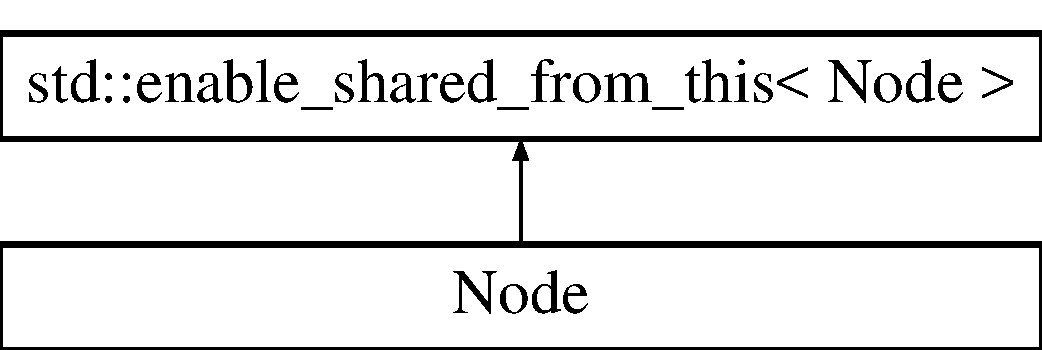
\includegraphics[height=2.000000cm]{classNode}
\end{center}
\end{figure}
\subsection*{Public Member Functions}
\begin{DoxyCompactItemize}
\item 
\hyperlink{classNode_ad7a34779cad45d997bfd6d3d8043c75f}{Node} ()
\item 
void \hyperlink{classNode_a68d5f074d4d9487384500bdcc80d489b}{draw} (glm\+::mat4 model, glm\+::mat4 \&view, glm\+::mat4 \&projection)
\item 
\hyperlink{Node_8hpp_ac189bcbe7762c82a1a30c219d6ebdf75}{p\+Node} \hyperlink{classNode_ac9fb91f489ca00c8e91f10eda66cfffe}{create\+\_\+child} ()
\item 
\hyperlink{Node_8hpp_ac189bcbe7762c82a1a30c219d6ebdf75}{p\+Node} \hyperlink{classNode_abdaf4340bd75b5621c0a75f18590476e}{remove\+\_\+child} (\hyperlink{Node_8hpp_ac189bcbe7762c82a1a30c219d6ebdf75}{p\+Node} \&child)
\item 
void \hyperlink{classNode_ac2eb884b8982645f6d7438025a60cbff}{set\+\_\+position} (G\+Lfloat x, G\+Lfloat y, G\+Lfloat z)
\item 
void \hyperlink{classNode_a056137e4e51a4587490451c1dbefb23e}{set\+\_\+position} (glm\+::vec3 position)
\item 
void \hyperlink{classNode_a02c9938a7714e058c07b453552b6ad6d}{set\+\_\+orientation} (G\+Lfloat x, G\+Lfloat y, G\+Lfloat z, G\+Lfloat w)
\item 
void \hyperlink{classNode_a37476444f918a2e23f6229845dc44f6e}{set\+\_\+orientation} (glm\+::quat rotation)
\item 
void \hyperlink{classNode_a4fe91fd27202fb20d219ba476e6ff3a1}{set\+\_\+orientation} (glm\+::vec3 axis, G\+Lfloat w)
\item 
void \hyperlink{classNode_a6bdc035991cc9518b6139d34e32603a8}{yaw} (G\+Lfloat yaw)
\item 
void \hyperlink{classNode_aa88c3fa387ddc4c8991c20f6e901a247}{pitch} (G\+Lfloat pitch)
\item 
void \hyperlink{classNode_a078e56eb86c4049d9c282485b8439cf1}{roll} (G\+Lfloat roll)
\item 
void \hyperlink{classNode_a0c403c5effe407349dea4039eb2987be}{translate} (G\+Lfloat x, G\+Lfloat y, G\+Lfloat z)
\item 
void \hyperlink{classNode_abfa9ae84c73cd9197dd27aee75e595ce}{translate} (glm\+::vec3 vec)
\item 
void \hyperlink{classNode_a3faec015e7b7739ee810a44540aa2250}{set\+\_\+scale} (glm\+::vec3 scale)
\item 
void \hyperlink{classNode_ad136d4dc5400c4091ea22e6d24a445e5}{set\+\_\+scale} (G\+Lfloat x, G\+Lfloat y, G\+Lfloat z)
\item 
void \hyperlink{classNode_a778a680844ceddae2c5fd76755a5d99d}{attach\+\_\+entity} (\hyperlink{Entity_8hpp_ae424507ba09ae72f3c142ce741f3a1e7}{p\+Entity} \&entity)
\item 
\hyperlink{Entity_8hpp_ae424507ba09ae72f3c142ce741f3a1e7}{p\+Entity} \hyperlink{classNode_ad27c6c51391f092f6dc2fdea545f283d}{remove\+\_\+entity} ()
\end{DoxyCompactItemize}
\subsection*{Private Attributes}
\begin{DoxyCompactItemize}
\item 
\hyperlink{Entity_8hpp_ae424507ba09ae72f3c142ce741f3a1e7}{p\+Entity} \hyperlink{classNode_a3368ad7073fca05b90d0f38bfdea3cd5}{\+\_\+entity}
\item 
std\+::weak\+\_\+ptr$<$ \hyperlink{classNode}{Node} $>$ \hyperlink{classNode_a56087f97d2017476c226457a40140d20}{\+\_\+parent}
\item 
std\+::unordered\+\_\+set$<$ \hyperlink{Node_8hpp_ac189bcbe7762c82a1a30c219d6ebdf75}{p\+Node} $>$ \hyperlink{classNode_a6ee8ca308823ce214bfcb016f5bc7879}{\+\_\+children}
\item 
glm\+::vec3 \hyperlink{classNode_a69c878f3787faea652415b389977894d}{\+\_\+position}
\item 
glm\+::quat \hyperlink{classNode_a8ca75f9f976a292c9f56c881162ee606}{\+\_\+rotation}
\item 
glm\+::vec3 \hyperlink{classNode_a87179723de57ea9bdcf179ee5164deb3}{\+\_\+scale}
\end{DoxyCompactItemize}


\subsection{Constructor \& Destructor Documentation}
\index{Node@{Node}!Node@{Node}}
\index{Node@{Node}!Node@{Node}}
\subsubsection[{\texorpdfstring{Node()}{Node()}}]{\setlength{\rightskip}{0pt plus 5cm}Node\+::\+Node (
\begin{DoxyParamCaption}
{}
\end{DoxyParamCaption}
)}\hypertarget{classNode_ad7a34779cad45d997bfd6d3d8043c75f}{}\label{classNode_ad7a34779cad45d997bfd6d3d8043c75f}


\subsection{Member Function Documentation}
\index{Node@{Node}!attach\+\_\+entity@{attach\+\_\+entity}}
\index{attach\+\_\+entity@{attach\+\_\+entity}!Node@{Node}}
\subsubsection[{\texorpdfstring{attach\+\_\+entity(p\+Entity \&entity)}{attach_entity(pEntity &entity)}}]{\setlength{\rightskip}{0pt plus 5cm}void Node\+::attach\+\_\+entity (
\begin{DoxyParamCaption}
\item[{{\bf p\+Entity} \&}]{entity}
\end{DoxyParamCaption}
)}\hypertarget{classNode_a778a680844ceddae2c5fd76755a5d99d}{}\label{classNode_a778a680844ceddae2c5fd76755a5d99d}
\index{Node@{Node}!create\+\_\+child@{create\+\_\+child}}
\index{create\+\_\+child@{create\+\_\+child}!Node@{Node}}
\subsubsection[{\texorpdfstring{create\+\_\+child()}{create_child()}}]{\setlength{\rightskip}{0pt plus 5cm}{\bf p\+Node} Node\+::create\+\_\+child (
\begin{DoxyParamCaption}
{}
\end{DoxyParamCaption}
)}\hypertarget{classNode_ac9fb91f489ca00c8e91f10eda66cfffe}{}\label{classNode_ac9fb91f489ca00c8e91f10eda66cfffe}
\index{Node@{Node}!draw@{draw}}
\index{draw@{draw}!Node@{Node}}
\subsubsection[{\texorpdfstring{draw(glm\+::mat4 model, glm\+::mat4 \&view, glm\+::mat4 \&projection)}{draw(glm::mat4 model, glm::mat4 &view, glm::mat4 &projection)}}]{\setlength{\rightskip}{0pt plus 5cm}void Node\+::draw (
\begin{DoxyParamCaption}
\item[{glm\+::mat4}]{model, }
\item[{glm\+::mat4 \&}]{view, }
\item[{glm\+::mat4 \&}]{projection}
\end{DoxyParamCaption}
)}\hypertarget{classNode_a68d5f074d4d9487384500bdcc80d489b}{}\label{classNode_a68d5f074d4d9487384500bdcc80d489b}
\index{Node@{Node}!pitch@{pitch}}
\index{pitch@{pitch}!Node@{Node}}
\subsubsection[{\texorpdfstring{pitch(\+G\+Lfloat pitch)}{pitch(GLfloat pitch)}}]{\setlength{\rightskip}{0pt plus 5cm}void Node\+::pitch (
\begin{DoxyParamCaption}
\item[{G\+Lfloat}]{pitch}
\end{DoxyParamCaption}
)}\hypertarget{classNode_aa88c3fa387ddc4c8991c20f6e901a247}{}\label{classNode_aa88c3fa387ddc4c8991c20f6e901a247}
\index{Node@{Node}!remove\+\_\+child@{remove\+\_\+child}}
\index{remove\+\_\+child@{remove\+\_\+child}!Node@{Node}}
\subsubsection[{\texorpdfstring{remove\+\_\+child(p\+Node \&child)}{remove_child(pNode &child)}}]{\setlength{\rightskip}{0pt plus 5cm}{\bf p\+Node} Node\+::remove\+\_\+child (
\begin{DoxyParamCaption}
\item[{{\bf p\+Node} \&}]{child}
\end{DoxyParamCaption}
)}\hypertarget{classNode_abdaf4340bd75b5621c0a75f18590476e}{}\label{classNode_abdaf4340bd75b5621c0a75f18590476e}
\index{Node@{Node}!remove\+\_\+entity@{remove\+\_\+entity}}
\index{remove\+\_\+entity@{remove\+\_\+entity}!Node@{Node}}
\subsubsection[{\texorpdfstring{remove\+\_\+entity()}{remove_entity()}}]{\setlength{\rightskip}{0pt plus 5cm}{\bf p\+Entity} Node\+::remove\+\_\+entity (
\begin{DoxyParamCaption}
{}
\end{DoxyParamCaption}
)}\hypertarget{classNode_ad27c6c51391f092f6dc2fdea545f283d}{}\label{classNode_ad27c6c51391f092f6dc2fdea545f283d}
\index{Node@{Node}!roll@{roll}}
\index{roll@{roll}!Node@{Node}}
\subsubsection[{\texorpdfstring{roll(\+G\+Lfloat roll)}{roll(GLfloat roll)}}]{\setlength{\rightskip}{0pt plus 5cm}void Node\+::roll (
\begin{DoxyParamCaption}
\item[{G\+Lfloat}]{roll}
\end{DoxyParamCaption}
)}\hypertarget{classNode_a078e56eb86c4049d9c282485b8439cf1}{}\label{classNode_a078e56eb86c4049d9c282485b8439cf1}
\index{Node@{Node}!set\+\_\+orientation@{set\+\_\+orientation}}
\index{set\+\_\+orientation@{set\+\_\+orientation}!Node@{Node}}
\subsubsection[{\texorpdfstring{set\+\_\+orientation(\+G\+Lfloat x, G\+Lfloat y, G\+Lfloat z, G\+Lfloat w)}{set_orientation(GLfloat x, GLfloat y, GLfloat z, GLfloat w)}}]{\setlength{\rightskip}{0pt plus 5cm}void Node\+::set\+\_\+orientation (
\begin{DoxyParamCaption}
\item[{G\+Lfloat}]{x, }
\item[{G\+Lfloat}]{y, }
\item[{G\+Lfloat}]{z, }
\item[{G\+Lfloat}]{w}
\end{DoxyParamCaption}
)}\hypertarget{classNode_a02c9938a7714e058c07b453552b6ad6d}{}\label{classNode_a02c9938a7714e058c07b453552b6ad6d}
\index{Node@{Node}!set\+\_\+orientation@{set\+\_\+orientation}}
\index{set\+\_\+orientation@{set\+\_\+orientation}!Node@{Node}}
\subsubsection[{\texorpdfstring{set\+\_\+orientation(glm\+::quat rotation)}{set_orientation(glm::quat rotation)}}]{\setlength{\rightskip}{0pt plus 5cm}void Node\+::set\+\_\+orientation (
\begin{DoxyParamCaption}
\item[{glm\+::quat}]{rotation}
\end{DoxyParamCaption}
)}\hypertarget{classNode_a37476444f918a2e23f6229845dc44f6e}{}\label{classNode_a37476444f918a2e23f6229845dc44f6e}
\index{Node@{Node}!set\+\_\+orientation@{set\+\_\+orientation}}
\index{set\+\_\+orientation@{set\+\_\+orientation}!Node@{Node}}
\subsubsection[{\texorpdfstring{set\+\_\+orientation(glm\+::vec3 axis, G\+Lfloat w)}{set_orientation(glm::vec3 axis, GLfloat w)}}]{\setlength{\rightskip}{0pt plus 5cm}void Node\+::set\+\_\+orientation (
\begin{DoxyParamCaption}
\item[{glm\+::vec3}]{axis, }
\item[{G\+Lfloat}]{w}
\end{DoxyParamCaption}
)}\hypertarget{classNode_a4fe91fd27202fb20d219ba476e6ff3a1}{}\label{classNode_a4fe91fd27202fb20d219ba476e6ff3a1}
\index{Node@{Node}!set\+\_\+position@{set\+\_\+position}}
\index{set\+\_\+position@{set\+\_\+position}!Node@{Node}}
\subsubsection[{\texorpdfstring{set\+\_\+position(\+G\+Lfloat x, G\+Lfloat y, G\+Lfloat z)}{set_position(GLfloat x, GLfloat y, GLfloat z)}}]{\setlength{\rightskip}{0pt plus 5cm}void Node\+::set\+\_\+position (
\begin{DoxyParamCaption}
\item[{G\+Lfloat}]{x, }
\item[{G\+Lfloat}]{y, }
\item[{G\+Lfloat}]{z}
\end{DoxyParamCaption}
)}\hypertarget{classNode_ac2eb884b8982645f6d7438025a60cbff}{}\label{classNode_ac2eb884b8982645f6d7438025a60cbff}
\index{Node@{Node}!set\+\_\+position@{set\+\_\+position}}
\index{set\+\_\+position@{set\+\_\+position}!Node@{Node}}
\subsubsection[{\texorpdfstring{set\+\_\+position(glm\+::vec3 position)}{set_position(glm::vec3 position)}}]{\setlength{\rightskip}{0pt plus 5cm}void Node\+::set\+\_\+position (
\begin{DoxyParamCaption}
\item[{glm\+::vec3}]{position}
\end{DoxyParamCaption}
)}\hypertarget{classNode_a056137e4e51a4587490451c1dbefb23e}{}\label{classNode_a056137e4e51a4587490451c1dbefb23e}
\index{Node@{Node}!set\+\_\+scale@{set\+\_\+scale}}
\index{set\+\_\+scale@{set\+\_\+scale}!Node@{Node}}
\subsubsection[{\texorpdfstring{set\+\_\+scale(glm\+::vec3 scale)}{set_scale(glm::vec3 scale)}}]{\setlength{\rightskip}{0pt plus 5cm}void Node\+::set\+\_\+scale (
\begin{DoxyParamCaption}
\item[{glm\+::vec3}]{scale}
\end{DoxyParamCaption}
)}\hypertarget{classNode_a3faec015e7b7739ee810a44540aa2250}{}\label{classNode_a3faec015e7b7739ee810a44540aa2250}
\index{Node@{Node}!set\+\_\+scale@{set\+\_\+scale}}
\index{set\+\_\+scale@{set\+\_\+scale}!Node@{Node}}
\subsubsection[{\texorpdfstring{set\+\_\+scale(\+G\+Lfloat x, G\+Lfloat y, G\+Lfloat z)}{set_scale(GLfloat x, GLfloat y, GLfloat z)}}]{\setlength{\rightskip}{0pt plus 5cm}void Node\+::set\+\_\+scale (
\begin{DoxyParamCaption}
\item[{G\+Lfloat}]{x, }
\item[{G\+Lfloat}]{y, }
\item[{G\+Lfloat}]{z}
\end{DoxyParamCaption}
)}\hypertarget{classNode_ad136d4dc5400c4091ea22e6d24a445e5}{}\label{classNode_ad136d4dc5400c4091ea22e6d24a445e5}
\index{Node@{Node}!translate@{translate}}
\index{translate@{translate}!Node@{Node}}
\subsubsection[{\texorpdfstring{translate(\+G\+Lfloat x, G\+Lfloat y, G\+Lfloat z)}{translate(GLfloat x, GLfloat y, GLfloat z)}}]{\setlength{\rightskip}{0pt plus 5cm}void Node\+::translate (
\begin{DoxyParamCaption}
\item[{G\+Lfloat}]{x, }
\item[{G\+Lfloat}]{y, }
\item[{G\+Lfloat}]{z}
\end{DoxyParamCaption}
)}\hypertarget{classNode_a0c403c5effe407349dea4039eb2987be}{}\label{classNode_a0c403c5effe407349dea4039eb2987be}
\index{Node@{Node}!translate@{translate}}
\index{translate@{translate}!Node@{Node}}
\subsubsection[{\texorpdfstring{translate(glm\+::vec3 vec)}{translate(glm::vec3 vec)}}]{\setlength{\rightskip}{0pt plus 5cm}void Node\+::translate (
\begin{DoxyParamCaption}
\item[{glm\+::vec3}]{vec}
\end{DoxyParamCaption}
)}\hypertarget{classNode_abfa9ae84c73cd9197dd27aee75e595ce}{}\label{classNode_abfa9ae84c73cd9197dd27aee75e595ce}
\index{Node@{Node}!yaw@{yaw}}
\index{yaw@{yaw}!Node@{Node}}
\subsubsection[{\texorpdfstring{yaw(\+G\+Lfloat yaw)}{yaw(GLfloat yaw)}}]{\setlength{\rightskip}{0pt plus 5cm}void Node\+::yaw (
\begin{DoxyParamCaption}
\item[{G\+Lfloat}]{yaw}
\end{DoxyParamCaption}
)}\hypertarget{classNode_a6bdc035991cc9518b6139d34e32603a8}{}\label{classNode_a6bdc035991cc9518b6139d34e32603a8}


\subsection{Member Data Documentation}
\index{Node@{Node}!\+\_\+children@{\+\_\+children}}
\index{\+\_\+children@{\+\_\+children}!Node@{Node}}
\subsubsection[{\texorpdfstring{\+\_\+children}{_children}}]{\setlength{\rightskip}{0pt plus 5cm}std\+::unordered\+\_\+set$<${\bf p\+Node}$>$ Node\+::\+\_\+children\hspace{0.3cm}{\ttfamily [private]}}\hypertarget{classNode_a6ee8ca308823ce214bfcb016f5bc7879}{}\label{classNode_a6ee8ca308823ce214bfcb016f5bc7879}
\index{Node@{Node}!\+\_\+entity@{\+\_\+entity}}
\index{\+\_\+entity@{\+\_\+entity}!Node@{Node}}
\subsubsection[{\texorpdfstring{\+\_\+entity}{_entity}}]{\setlength{\rightskip}{0pt plus 5cm}{\bf p\+Entity} Node\+::\+\_\+entity\hspace{0.3cm}{\ttfamily [private]}}\hypertarget{classNode_a3368ad7073fca05b90d0f38bfdea3cd5}{}\label{classNode_a3368ad7073fca05b90d0f38bfdea3cd5}
\index{Node@{Node}!\+\_\+parent@{\+\_\+parent}}
\index{\+\_\+parent@{\+\_\+parent}!Node@{Node}}
\subsubsection[{\texorpdfstring{\+\_\+parent}{_parent}}]{\setlength{\rightskip}{0pt plus 5cm}std\+::weak\+\_\+ptr$<${\bf Node}$>$ Node\+::\+\_\+parent\hspace{0.3cm}{\ttfamily [private]}}\hypertarget{classNode_a56087f97d2017476c226457a40140d20}{}\label{classNode_a56087f97d2017476c226457a40140d20}
\index{Node@{Node}!\+\_\+position@{\+\_\+position}}
\index{\+\_\+position@{\+\_\+position}!Node@{Node}}
\subsubsection[{\texorpdfstring{\+\_\+position}{_position}}]{\setlength{\rightskip}{0pt plus 5cm}glm\+::vec3 Node\+::\+\_\+position\hspace{0.3cm}{\ttfamily [private]}}\hypertarget{classNode_a69c878f3787faea652415b389977894d}{}\label{classNode_a69c878f3787faea652415b389977894d}
\index{Node@{Node}!\+\_\+rotation@{\+\_\+rotation}}
\index{\+\_\+rotation@{\+\_\+rotation}!Node@{Node}}
\subsubsection[{\texorpdfstring{\+\_\+rotation}{_rotation}}]{\setlength{\rightskip}{0pt plus 5cm}glm\+::quat Node\+::\+\_\+rotation\hspace{0.3cm}{\ttfamily [private]}}\hypertarget{classNode_a8ca75f9f976a292c9f56c881162ee606}{}\label{classNode_a8ca75f9f976a292c9f56c881162ee606}
\index{Node@{Node}!\+\_\+scale@{\+\_\+scale}}
\index{\+\_\+scale@{\+\_\+scale}!Node@{Node}}
\subsubsection[{\texorpdfstring{\+\_\+scale}{_scale}}]{\setlength{\rightskip}{0pt plus 5cm}glm\+::vec3 Node\+::\+\_\+scale\hspace{0.3cm}{\ttfamily [private]}}\hypertarget{classNode_a87179723de57ea9bdcf179ee5164deb3}{}\label{classNode_a87179723de57ea9bdcf179ee5164deb3}


The documentation for this class was generated from the following files\+:\begin{DoxyCompactItemize}
\item 
src/\hyperlink{Node_8hpp}{Node.\+hpp}\item 
src/\hyperlink{Node_8cpp}{Node.\+cpp}\end{DoxyCompactItemize}

\hypertarget{classRootNode}{}\section{Root\+Node Class Reference}
\label{classRootNode}\index{Root\+Node@{Root\+Node}}


{\ttfamily \#include $<$Root\+Node.\+hpp$>$}



The documentation for this class was generated from the following file\+:\begin{DoxyCompactItemize}
\item 
src/\hyperlink{RootNode_8hpp}{Root\+Node.\+hpp}\end{DoxyCompactItemize}

\hypertarget{classSceneGraph}{}\section{Scene\+Graph Class Reference}
\label{classSceneGraph}\index{Scene\+Graph@{Scene\+Graph}}


{\ttfamily \#include $<$Scene\+Graph.\+hpp$>$}

\subsection*{Public Member Functions}
\begin{DoxyCompactItemize}
\item 
\hyperlink{Node_8hpp_ac189bcbe7762c82a1a30c219d6ebdf75}{p\+Node} \hyperlink{classSceneGraph_acbfb3a25078b31f41a2373bf2f7747ae}{create\+\_\+child\+\_\+node} ()
\item 
void \hyperlink{classSceneGraph_a02138d9b44c12b1998141f7890421aee}{draw} (glm\+::mat4 \&view, glm\+::mat4 \&projection)
\item 
void \hyperlink{classSceneGraph_af16410fa90b4739b5d26a424d7857713}{set\+\_\+ambient\+\_\+light} (glm\+::vec3 color)
\end{DoxyCompactItemize}
\subsection*{Static Public Member Functions}
\begin{DoxyCompactItemize}
\item 
static \hyperlink{SceneGraph_8hpp_a12ad25ef584ef693808fd28bbff29c81}{p\+Scene\+Graph} \hyperlink{classSceneGraph_a3cd0423e853a2f8ea5ef59a1423f163b}{singleton} ()
\end{DoxyCompactItemize}


\subsection{Member Function Documentation}
\index{Scene\+Graph@{Scene\+Graph}!create\+\_\+child\+\_\+node@{create\+\_\+child\+\_\+node}}
\index{create\+\_\+child\+\_\+node@{create\+\_\+child\+\_\+node}!Scene\+Graph@{Scene\+Graph}}
\subsubsection[{\texorpdfstring{create\+\_\+child\+\_\+node()}{create_child_node()}}]{\setlength{\rightskip}{0pt plus 5cm}{\bf p\+Node} Scene\+Graph\+::create\+\_\+child\+\_\+node (
\begin{DoxyParamCaption}
{}
\end{DoxyParamCaption}
)}\hypertarget{classSceneGraph_acbfb3a25078b31f41a2373bf2f7747ae}{}\label{classSceneGraph_acbfb3a25078b31f41a2373bf2f7747ae}
\index{Scene\+Graph@{Scene\+Graph}!draw@{draw}}
\index{draw@{draw}!Scene\+Graph@{Scene\+Graph}}
\subsubsection[{\texorpdfstring{draw(glm\+::mat4 \&view, glm\+::mat4 \&projection)}{draw(glm::mat4 &view, glm::mat4 &projection)}}]{\setlength{\rightskip}{0pt plus 5cm}void Scene\+Graph\+::draw (
\begin{DoxyParamCaption}
\item[{glm\+::mat4 \&}]{view, }
\item[{glm\+::mat4 \&}]{projection}
\end{DoxyParamCaption}
)}\hypertarget{classSceneGraph_a02138d9b44c12b1998141f7890421aee}{}\label{classSceneGraph_a02138d9b44c12b1998141f7890421aee}
\index{Scene\+Graph@{Scene\+Graph}!set\+\_\+ambient\+\_\+light@{set\+\_\+ambient\+\_\+light}}
\index{set\+\_\+ambient\+\_\+light@{set\+\_\+ambient\+\_\+light}!Scene\+Graph@{Scene\+Graph}}
\subsubsection[{\texorpdfstring{set\+\_\+ambient\+\_\+light(glm\+::vec3 color)}{set_ambient_light(glm::vec3 color)}}]{\setlength{\rightskip}{0pt plus 5cm}void Scene\+Graph\+::set\+\_\+ambient\+\_\+light (
\begin{DoxyParamCaption}
\item[{glm\+::vec3}]{color}
\end{DoxyParamCaption}
)}\hypertarget{classSceneGraph_af16410fa90b4739b5d26a424d7857713}{}\label{classSceneGraph_af16410fa90b4739b5d26a424d7857713}
\index{Scene\+Graph@{Scene\+Graph}!singleton@{singleton}}
\index{singleton@{singleton}!Scene\+Graph@{Scene\+Graph}}
\subsubsection[{\texorpdfstring{singleton()}{singleton()}}]{\setlength{\rightskip}{0pt plus 5cm}{\bf p\+Scene\+Graph} Scene\+Graph\+::singleton (
\begin{DoxyParamCaption}
{}
\end{DoxyParamCaption}
)\hspace{0.3cm}{\ttfamily [static]}}\hypertarget{classSceneGraph_a3cd0423e853a2f8ea5ef59a1423f163b}{}\label{classSceneGraph_a3cd0423e853a2f8ea5ef59a1423f163b}


The documentation for this class was generated from the following files\+:\begin{DoxyCompactItemize}
\item 
src/\hyperlink{SceneGraph_8hpp}{Scene\+Graph.\+hpp}\item 
src/\hyperlink{SceneGraph_8cpp}{Scene\+Graph.\+cpp}\end{DoxyCompactItemize}

\hypertarget{classShader}{}\section{Shader Class Reference}
\label{classShader}\index{Shader@{Shader}}


{\ttfamily \#include $<$Shader.\+hpp$>$}

\subsection*{Public Member Functions}
\begin{DoxyCompactItemize}
\item 
\hyperlink{classShader_a03421a8419cdad4b84cf58ecdb156879}{Shader} (const G\+Lchar $\ast$vertex\+Path, const G\+Lchar $\ast$fragment\+Path)
\item 
void \hyperlink{classShader_a870fa9f13d69e558815d6fd351a469dc}{use} ()
\end{DoxyCompactItemize}
\subsection*{Public Attributes}
\begin{DoxyCompactItemize}
\item 
G\+Luint \hyperlink{classShader_a5978edd53515ba3e8035a13ceb4404ef}{m\+Program}
\end{DoxyCompactItemize}


\subsection{Constructor \& Destructor Documentation}
\index{Shader@{Shader}!Shader@{Shader}}
\index{Shader@{Shader}!Shader@{Shader}}
\subsubsection[{\texorpdfstring{Shader(const G\+Lchar $\ast$vertex\+Path, const G\+Lchar $\ast$fragment\+Path)}{Shader(const GLchar *vertexPath, const GLchar *fragmentPath)}}]{\setlength{\rightskip}{0pt plus 5cm}Shader\+::\+Shader (
\begin{DoxyParamCaption}
\item[{const G\+Lchar $\ast$}]{vertex\+Path, }
\item[{const G\+Lchar $\ast$}]{fragment\+Path}
\end{DoxyParamCaption}
)}\hypertarget{classShader_a03421a8419cdad4b84cf58ecdb156879}{}\label{classShader_a03421a8419cdad4b84cf58ecdb156879}


\subsection{Member Function Documentation}
\index{Shader@{Shader}!use@{use}}
\index{use@{use}!Shader@{Shader}}
\subsubsection[{\texorpdfstring{use()}{use()}}]{\setlength{\rightskip}{0pt plus 5cm}void Shader\+::use (
\begin{DoxyParamCaption}
{}
\end{DoxyParamCaption}
)}\hypertarget{classShader_a870fa9f13d69e558815d6fd351a469dc}{}\label{classShader_a870fa9f13d69e558815d6fd351a469dc}


\subsection{Member Data Documentation}
\index{Shader@{Shader}!m\+Program@{m\+Program}}
\index{m\+Program@{m\+Program}!Shader@{Shader}}
\subsubsection[{\texorpdfstring{m\+Program}{mProgram}}]{\setlength{\rightskip}{0pt plus 5cm}G\+Luint Shader\+::m\+Program}\hypertarget{classShader_a5978edd53515ba3e8035a13ceb4404ef}{}\label{classShader_a5978edd53515ba3e8035a13ceb4404ef}


The documentation for this class was generated from the following files\+:\begin{DoxyCompactItemize}
\item 
src/\hyperlink{Shader_8hpp}{Shader.\+hpp}\item 
src/\hyperlink{Shader_8cpp}{Shader.\+cpp}\end{DoxyCompactItemize}

\hypertarget{classTexture}{}\section{Texture Class Reference}
\label{classTexture}\index{Texture@{Texture}}


{\ttfamily \#include $<$Mesh.\+hpp$>$}

\subsection*{Public Types}
\begin{DoxyCompactItemize}
\item 
enum \hyperlink{classTexture_a9d0b09cfb795f9553db6a4eab396bef9}{Type} \{ \hyperlink{classTexture_a9d0b09cfb795f9553db6a4eab396bef9a30c8ec5c46cfae607655ca4b913b87df}{D\+I\+F\+F\+U\+SE}, 
\hyperlink{classTexture_a9d0b09cfb795f9553db6a4eab396bef9a0dd9b82cf1e92a09e1a78bd0014cbbea}{S\+P\+E\+C\+U\+L\+AR}
 \}
\end{DoxyCompactItemize}
\subsection*{Public Member Functions}
\begin{DoxyCompactItemize}
\item 
std\+::string \hyperlink{classTexture_aac49cba59991aaab1c2d6e6d186beefb}{to\+String} ()
\end{DoxyCompactItemize}
\subsection*{Public Attributes}
\begin{DoxyCompactItemize}
\item 
G\+Luint \hyperlink{classTexture_ad34618c2c7f986a956453d1208a1912b}{m\+ID}
\item 
\hyperlink{classTexture_a9d0b09cfb795f9553db6a4eab396bef9}{Type} \hyperlink{classTexture_a25fca6d1c32a423f83decd7f738864ce}{m\+Type}
\item 
ai\+String \hyperlink{classTexture_a637c7fd5c6fab7b1b2cbc91d8b5a9bba}{m\+Path}
\end{DoxyCompactItemize}


\subsection{Member Enumeration Documentation}
\index{Texture@{Texture}!Type@{Type}}
\index{Type@{Type}!Texture@{Texture}}
\subsubsection[{\texorpdfstring{Type}{Type}}]{\setlength{\rightskip}{0pt plus 5cm}enum {\bf Texture\+::\+Type}}\hypertarget{classTexture_a9d0b09cfb795f9553db6a4eab396bef9}{}\label{classTexture_a9d0b09cfb795f9553db6a4eab396bef9}
\begin{Desc}
\item[Enumerator]\par
\begin{description}
\index{D\+I\+F\+F\+U\+SE@{D\+I\+F\+F\+U\+SE}!Texture@{Texture}}\index{Texture@{Texture}!D\+I\+F\+F\+U\+SE@{D\+I\+F\+F\+U\+SE}}\item[{\em 
D\+I\+F\+F\+U\+SE\hypertarget{classTexture_a9d0b09cfb795f9553db6a4eab396bef9a30c8ec5c46cfae607655ca4b913b87df}{}\label{classTexture_a9d0b09cfb795f9553db6a4eab396bef9a30c8ec5c46cfae607655ca4b913b87df}
}]\index{S\+P\+E\+C\+U\+L\+AR@{S\+P\+E\+C\+U\+L\+AR}!Texture@{Texture}}\index{Texture@{Texture}!S\+P\+E\+C\+U\+L\+AR@{S\+P\+E\+C\+U\+L\+AR}}\item[{\em 
S\+P\+E\+C\+U\+L\+AR\hypertarget{classTexture_a9d0b09cfb795f9553db6a4eab396bef9a0dd9b82cf1e92a09e1a78bd0014cbbea}{}\label{classTexture_a9d0b09cfb795f9553db6a4eab396bef9a0dd9b82cf1e92a09e1a78bd0014cbbea}
}]\end{description}
\end{Desc}


\subsection{Member Function Documentation}
\index{Texture@{Texture}!to\+String@{to\+String}}
\index{to\+String@{to\+String}!Texture@{Texture}}
\subsubsection[{\texorpdfstring{to\+String()}{toString()}}]{\setlength{\rightskip}{0pt plus 5cm}std\+::string Texture\+::to\+String (
\begin{DoxyParamCaption}
{}
\end{DoxyParamCaption}
)}\hypertarget{classTexture_aac49cba59991aaab1c2d6e6d186beefb}{}\label{classTexture_aac49cba59991aaab1c2d6e6d186beefb}


\subsection{Member Data Documentation}
\index{Texture@{Texture}!m\+ID@{m\+ID}}
\index{m\+ID@{m\+ID}!Texture@{Texture}}
\subsubsection[{\texorpdfstring{m\+ID}{mID}}]{\setlength{\rightskip}{0pt plus 5cm}G\+Luint Texture\+::m\+ID}\hypertarget{classTexture_ad34618c2c7f986a956453d1208a1912b}{}\label{classTexture_ad34618c2c7f986a956453d1208a1912b}
\index{Texture@{Texture}!m\+Path@{m\+Path}}
\index{m\+Path@{m\+Path}!Texture@{Texture}}
\subsubsection[{\texorpdfstring{m\+Path}{mPath}}]{\setlength{\rightskip}{0pt plus 5cm}ai\+String Texture\+::m\+Path}\hypertarget{classTexture_a637c7fd5c6fab7b1b2cbc91d8b5a9bba}{}\label{classTexture_a637c7fd5c6fab7b1b2cbc91d8b5a9bba}
\index{Texture@{Texture}!m\+Type@{m\+Type}}
\index{m\+Type@{m\+Type}!Texture@{Texture}}
\subsubsection[{\texorpdfstring{m\+Type}{mType}}]{\setlength{\rightskip}{0pt plus 5cm}{\bf Type} Texture\+::m\+Type}\hypertarget{classTexture_a25fca6d1c32a423f83decd7f738864ce}{}\label{classTexture_a25fca6d1c32a423f83decd7f738864ce}


The documentation for this class was generated from the following files\+:\begin{DoxyCompactItemize}
\item 
src/\hyperlink{Mesh_8hpp}{Mesh.\+hpp}\item 
src/\hyperlink{Mesh_8cpp}{Mesh.\+cpp}\end{DoxyCompactItemize}

\hypertarget{structVertex}{}\section{Vertex Struct Reference}
\label{structVertex}\index{Vertex@{Vertex}}


{\ttfamily \#include $<$Mesh.\+hpp$>$}

\subsection*{Public Attributes}
\begin{DoxyCompactItemize}
\item 
glm\+::vec3 \hyperlink{structVertex_a1b8266b61e52e83271623e40b9bbba07}{m\+Position}
\item 
glm\+::vec3 \hyperlink{structVertex_a1954547988e2fed7e7e936eb74e09cae}{m\+Normal}
\item 
glm\+::vec2 \hyperlink{structVertex_a2cff7003a258a96a3a26314024655790}{m\+Tex\+Coords}
\end{DoxyCompactItemize}


\subsection{Member Data Documentation}
\index{Vertex@{Vertex}!m\+Normal@{m\+Normal}}
\index{m\+Normal@{m\+Normal}!Vertex@{Vertex}}
\subsubsection[{\texorpdfstring{m\+Normal}{mNormal}}]{\setlength{\rightskip}{0pt plus 5cm}glm\+::vec3 Vertex\+::m\+Normal}\hypertarget{structVertex_a1954547988e2fed7e7e936eb74e09cae}{}\label{structVertex_a1954547988e2fed7e7e936eb74e09cae}
\index{Vertex@{Vertex}!m\+Position@{m\+Position}}
\index{m\+Position@{m\+Position}!Vertex@{Vertex}}
\subsubsection[{\texorpdfstring{m\+Position}{mPosition}}]{\setlength{\rightskip}{0pt plus 5cm}glm\+::vec3 Vertex\+::m\+Position}\hypertarget{structVertex_a1b8266b61e52e83271623e40b9bbba07}{}\label{structVertex_a1b8266b61e52e83271623e40b9bbba07}
\index{Vertex@{Vertex}!m\+Tex\+Coords@{m\+Tex\+Coords}}
\index{m\+Tex\+Coords@{m\+Tex\+Coords}!Vertex@{Vertex}}
\subsubsection[{\texorpdfstring{m\+Tex\+Coords}{mTexCoords}}]{\setlength{\rightskip}{0pt plus 5cm}glm\+::vec2 Vertex\+::m\+Tex\+Coords}\hypertarget{structVertex_a2cff7003a258a96a3a26314024655790}{}\label{structVertex_a2cff7003a258a96a3a26314024655790}


The documentation for this struct was generated from the following file\+:\begin{DoxyCompactItemize}
\item 
src/\hyperlink{Mesh_8hpp}{Mesh.\+hpp}\end{DoxyCompactItemize}

\chapter{File Documentation}
\hypertarget{Camera_8cpp}{\section{src/\-Camera.cpp File Reference}
\label{Camera_8cpp}\index{src/\-Camera.\-cpp@{src/\-Camera.\-cpp}}
}
{\ttfamily \#include \char`\"{}Camera.\-hpp\char`\"{}}\\*

\hypertarget{Camera_8hpp}{\section{src/\-Camera.hpp File Reference}
\label{Camera_8hpp}\index{src/\-Camera.\-hpp@{src/\-Camera.\-hpp}}
}
{\ttfamily \#include \char`\"{}Error.\-hpp\char`\"{}}\\*
{\ttfamily \#include $<$vector$>$}\\*
{\ttfamily \#include $<$G\-L/glew.\-h$>$}\\*
{\ttfamily \#include $<$glm/glm.\-hpp$>$}\\*
{\ttfamily \#include $<$glm/gtc/matrix\-\_\-transform.\-hpp$>$}\\*
\subsection*{Classes}
\begin{DoxyCompactItemize}
\item 
class \hyperlink{classCamera}{Camera}
\end{DoxyCompactItemize}

\hypertarget{Entity_8cpp}{}\section{src/\+Entity.cpp File Reference}
\label{Entity_8cpp}\index{src/\+Entity.\+cpp@{src/\+Entity.\+cpp}}
{\ttfamily \#include \char`\"{}Entity.\+hpp\char`\"{}}\\*
{\ttfamily \#include $<$iostream$>$}\\*

\hypertarget{Entity_8hpp}{}\section{src/\+Entity.hpp File Reference}
\label{Entity_8hpp}\index{src/\+Entity.\+hpp@{src/\+Entity.\+hpp}}
{\ttfamily \#include $<$glm/glm.\+hpp$>$}\\*
{\ttfamily \#include $<$glm/gtc/type\+\_\+ptr.\+hpp$>$}\\*
{\ttfamily \#include $<$memory$>$}\\*
{\ttfamily \#include \char`\"{}Model.\+hpp\char`\"{}}\\*
{\ttfamily \#include \char`\"{}Shader.\+hpp\char`\"{}}\\*
\subsection*{Classes}
\begin{DoxyCompactItemize}
\item 
class \hyperlink{classEntity}{Entity}
\end{DoxyCompactItemize}
\subsection*{Typedefs}
\begin{DoxyCompactItemize}
\item 
typedef std\+::shared\+\_\+ptr$<$ \hyperlink{classEntity}{Entity} $>$ \hyperlink{Entity_8hpp_ae424507ba09ae72f3c142ce741f3a1e7}{p\+Entity}
\end{DoxyCompactItemize}


\subsection{Typedef Documentation}
\index{Entity.\+hpp@{Entity.\+hpp}!p\+Entity@{p\+Entity}}
\index{p\+Entity@{p\+Entity}!Entity.\+hpp@{Entity.\+hpp}}
\subsubsection[{\texorpdfstring{p\+Entity}{pEntity}}]{\setlength{\rightskip}{0pt plus 5cm}typedef std\+::shared\+\_\+ptr$<${\bf Entity}$>$ {\bf p\+Entity}}\hypertarget{Entity_8hpp_ae424507ba09ae72f3c142ce741f3a1e7}{}\label{Entity_8hpp_ae424507ba09ae72f3c142ce741f3a1e7}

\hypertarget{Mesh_8cpp}{}\section{src/\+Mesh.cpp File Reference}
\label{Mesh_8cpp}\index{src/\+Mesh.\+cpp@{src/\+Mesh.\+cpp}}
{\ttfamily \#include \char`\"{}Mesh.\+hpp\char`\"{}}\\*
\subsection*{Namespaces}
\begin{DoxyCompactItemize}
\item 
 \hyperlink{namespaceLarp}{Larp}
\end{DoxyCompactItemize}

\hypertarget{Mesh_8hpp}{}\section{src/\+Mesh.hpp File Reference}
\label{Mesh_8hpp}\index{src/\+Mesh.\+hpp@{src/\+Mesh.\+hpp}}
{\ttfamily \#include \char`\"{}Shader.\+hpp\char`\"{}}\\*
{\ttfamily \#include $<$glm/glm.\+hpp$>$}\\*
{\ttfamily \#include $<$glm/gtc/matrix\+\_\+transform.\+hpp$>$}\\*
{\ttfamily \#include $<$S\+O\+I\+L.\+h$>$}\\*
{\ttfamily \#include $<$assimp/\+Importer.\+hpp$>$}\\*
{\ttfamily \#include $<$assimp/scene.\+h$>$}\\*
{\ttfamily \#include $<$assimp/postprocess.\+h$>$}\\*
{\ttfamily \#include $<$string$>$}\\*
{\ttfamily \#include $<$fstream$>$}\\*
{\ttfamily \#include $<$sstream$>$}\\*
{\ttfamily \#include $<$iostream$>$}\\*
{\ttfamily \#include $<$vector$>$}\\*
\subsection*{Classes}
\begin{DoxyCompactItemize}
\item 
struct \hyperlink{structVertex}{Vertex}
\item 
class \hyperlink{classTexture}{Texture}
\item 
class \hyperlink{classMesh}{Mesh}
\end{DoxyCompactItemize}
\subsection*{Functions}
\begin{DoxyCompactItemize}
\item 
G\+Lint \hyperlink{Mesh_8hpp_aeae4090b8c6535fcdbdc0374f490b9b9}{Texture\+From\+File} (const char $\ast$path, std\+::string directory)
\end{DoxyCompactItemize}


\subsection{Function Documentation}
\index{Mesh.\+hpp@{Mesh.\+hpp}!Texture\+From\+File@{Texture\+From\+File}}
\index{Texture\+From\+File@{Texture\+From\+File}!Mesh.\+hpp@{Mesh.\+hpp}}
\subsubsection[{\texorpdfstring{Texture\+From\+File(const char $\ast$path, std\+::string directory)}{TextureFromFile(const char *path, std::string directory)}}]{\setlength{\rightskip}{0pt plus 5cm}G\+Lint Texture\+From\+File (
\begin{DoxyParamCaption}
\item[{const char $\ast$}]{path, }
\item[{std\+::string}]{directory}
\end{DoxyParamCaption}
)}\hypertarget{Mesh_8hpp_aeae4090b8c6535fcdbdc0374f490b9b9}{}\label{Mesh_8hpp_aeae4090b8c6535fcdbdc0374f490b9b9}

\hypertarget{Model_8cpp}{\section{src/\-Model.cpp File Reference}
\label{Model_8cpp}\index{src/\-Model.\-cpp@{src/\-Model.\-cpp}}
}
{\ttfamily \#include \char`\"{}Model.\-hpp\char`\"{}}\\*
{\ttfamily \#include \char`\"{}Error.\-hpp\char`\"{}}\\*
\subsection*{Namespaces}
\begin{DoxyCompactItemize}
\item 
\hyperlink{namespaceLarp}{Larp}
\end{DoxyCompactItemize}

\hypertarget{Model_8hpp}{\section{src/\-Model.hpp File Reference}
\label{Model_8hpp}\index{src/\-Model.\-hpp@{src/\-Model.\-hpp}}
}
{\ttfamily \#include $<$assimp/\-Importer.\-hpp$>$}\\*
{\ttfamily \#include $<$assimp/scene.\-h$>$}\\*
{\ttfamily \#include $<$assimp/postprocess.\-h$>$}\\*
{\ttfamily \#include \char`\"{}Larp\-Prerequisites.\-hpp\char`\"{}}\\*
{\ttfamily \#include \char`\"{}Mesh.\-hpp\char`\"{}}\\*
\subsection*{Classes}
\begin{DoxyCompactItemize}
\item 
class \hyperlink{classLarp_1_1Model}{Larp\-::\-Model}
\end{DoxyCompactItemize}
\subsection*{Namespaces}
\begin{DoxyCompactItemize}
\item 
\hyperlink{namespaceLarp}{Larp}
\end{DoxyCompactItemize}

\hypertarget{Node_8cpp}{}\section{src/\+Node.cpp File Reference}
\label{Node_8cpp}\index{src/\+Node.\+cpp@{src/\+Node.\+cpp}}
{\ttfamily \#include \char`\"{}Node.\+hpp\char`\"{}}\\*
\subsection*{Namespaces}
\begin{DoxyCompactItemize}
\item 
 \hyperlink{namespaceLarp}{Larp}
\end{DoxyCompactItemize}

\hypertarget{Node_8hpp}{}\section{src/\+Node.hpp File Reference}
\label{Node_8hpp}\index{src/\+Node.\+hpp@{src/\+Node.\+hpp}}
{\ttfamily \#include $<$memory$>$}\\*
{\ttfamily \#include $<$unordered\+\_\+set$>$}\\*
{\ttfamily \#include $<$glm/glm.\+hpp$>$}\\*
{\ttfamily \#include $<$glm/gtc/quaternion.\+hpp$>$}\\*
{\ttfamily \#include $<$glm/gtx/quaternion.\+hpp$>$}\\*
{\ttfamily \#include \char`\"{}Larp\+Prerequisites.\+hpp\char`\"{}}\\*
{\ttfamily \#include \char`\"{}Entity.\+hpp\char`\"{}}\\*
\subsection*{Classes}
\begin{DoxyCompactItemize}
\item 
class \hyperlink{classLarp_1_1Node}{Larp\+::\+Node}
\end{DoxyCompactItemize}
\subsection*{Namespaces}
\begin{DoxyCompactItemize}
\item 
 \hyperlink{namespaceLarp}{Larp}
\end{DoxyCompactItemize}

\hypertarget{RootNode_8hpp}{}\section{src/\+Root\+Node.hpp File Reference}
\label{RootNode_8hpp}\index{src/\+Root\+Node.\+hpp@{src/\+Root\+Node.\+hpp}}
\subsection*{Classes}
\begin{DoxyCompactItemize}
\item 
class \hyperlink{classRootNode}{Root\+Node}
\end{DoxyCompactItemize}

\hypertarget{SceneGraph_8cpp}{}\section{src/\+Scene\+Graph.cpp File Reference}
\label{SceneGraph_8cpp}\index{src/\+Scene\+Graph.\+cpp@{src/\+Scene\+Graph.\+cpp}}
{\ttfamily \#include \char`\"{}Scene\+Graph.\+hpp\char`\"{}}\\*

\hypertarget{SceneGraph_8hpp}{}\section{src/\+Larp/\+Scene\+Graph.hpp File Reference}
\label{SceneGraph_8hpp}\index{src/\+Larp/\+Scene\+Graph.\+hpp@{src/\+Larp/\+Scene\+Graph.\+hpp}}
{\ttfamily \#include $<$algorithm$>$}\\*
{\ttfamily \#include $<$vector$>$}\\*
{\ttfamily \#include \char`\"{}Larp/\+Larp\+Prerequisites.\+hpp\char`\"{}}\\*
{\ttfamily \#include \char`\"{}Larp/\+Node.\+hpp\char`\"{}}\\*
{\ttfamily \#include \char`\"{}Larp/\+Sky\+Box.\+hpp\char`\"{}}\\*
\subsection*{Classes}
\begin{DoxyCompactItemize}
\item 
class \hyperlink{classLarp_1_1SceneGraph}{Larp\+::\+Scene\+Graph}
\end{DoxyCompactItemize}
\subsection*{Namespaces}
\begin{DoxyCompactItemize}
\item 
 \hyperlink{namespaceLarp}{Larp}
\end{DoxyCompactItemize}

\hypertarget{Shader_8cpp}{}\section{src/\+Shader.cpp File Reference}
\label{Shader_8cpp}\index{src/\+Shader.\+cpp@{src/\+Shader.\+cpp}}
{\ttfamily \#include \char`\"{}Shader.\+hpp\char`\"{}}\\*

\hypertarget{Shader_8hpp}{}\section{src/\+Larp/\+Shader.hpp File Reference}
\label{Shader_8hpp}\index{src/\+Larp/\+Shader.\+hpp@{src/\+Larp/\+Shader.\+hpp}}
{\ttfamily \#include \char`\"{}Larp\+Prerequisites.\+hpp\char`\"{}}\\*
{\ttfamily \#include $<$string$>$}\\*
{\ttfamily \#include $<$fstream$>$}\\*
{\ttfamily \#include $<$sstream$>$}\\*
{\ttfamily \#include $<$iostream$>$}\\*
\subsection*{Classes}
\begin{DoxyCompactItemize}
\item 
class \hyperlink{classLarp_1_1Shader}{Larp\+::\+Shader}
\end{DoxyCompactItemize}
\subsection*{Namespaces}
\begin{DoxyCompactItemize}
\item 
 \hyperlink{namespaceLarp}{Larp}
\end{DoxyCompactItemize}

\hypertarget{test_8cpp}{}\section{src/test.cpp File Reference}
\label{test_8cpp}\index{src/test.\+cpp@{src/test.\+cpp}}
{\ttfamily \#include $<$string$>$}\\*
{\ttfamily \#include $<$stdexcept$>$}\\*
{\ttfamily \#include $<$G\+L/glew.\+h$>$}\\*
{\ttfamily \#include $<$G\+L\+F\+W/glfw3.\+h$>$}\\*
{\ttfamily \#include \char`\"{}Larp/\+Larp\+Prerequisites.\+hpp\char`\"{}}\\*
{\ttfamily \#include \char`\"{}Larp/\+Configuration\+Loader.\+hpp\char`\"{}}\\*
{\ttfamily \#include \char`\"{}Larp/\+Model.\+hpp\char`\"{}}\\*
{\ttfamily \#include \char`\"{}Larp/\+Scene\+Graph.\+hpp\char`\"{}}\\*
{\ttfamily \#include \char`\"{}Larp/\+Shader.\+hpp\char`\"{}}\\*
{\ttfamily \#include \char`\"{}Larp/\+Sky\+Box.\+hpp\char`\"{}}\\*
{\ttfamily \#include \char`\"{}Camera.\+hpp\char`\"{}}\\*
{\ttfamily \#include \char`\"{}Physics\+Mesh\+Collider\+Builder.\+hpp\char`\"{}}\\*
{\ttfamily \#include \char`\"{}Physics\+Player\+Controller.\+hpp\char`\"{}}\\*
{\ttfamily \#include \char`\"{}Physics\+World.\+hpp\char`\"{}}\\*
{\ttfamily \#include $<$glm/glm.\+hpp$>$}\\*
{\ttfamily \#include $<$glm/gtc/matrix\+\_\+transform.\+hpp$>$}\\*
{\ttfamily \#include $<$glm/gtc/type\+\_\+ptr.\+hpp$>$}\\*
{\ttfamily \#include $<$S\+O\+I\+L.\+h$>$}\\*
{\ttfamily \#include $<$S\+D\+L/\+S\+D\+L.\+h$>$}\\*
\subsection*{Macros}
\begin{DoxyCompactItemize}
\item 
\#define \hyperlink{test_8cpp_abcde84ea0ef5f934384e4620f092c85a}{G\+L\+E\+W\+\_\+\+S\+T\+A\+T\+IC}
\end{DoxyCompactItemize}
\subsection*{Functions}
\begin{DoxyCompactItemize}
\item 
void \hyperlink{test_8cpp_aa48aaf412b9e33386433680c25b3883c}{key\+\_\+callback} (G\+L\+F\+Wwindow $\ast$window, int key, int scancode, int action, int mode)
\item 
void \hyperlink{test_8cpp_a06ad2502008f16fbcf01dfaa7f7bc9ea}{scroll\+\_\+callback} (G\+L\+F\+Wwindow $\ast$window, double xoffset, double yoffset)
\item 
void \hyperlink{test_8cpp_af4ca2891044ac10a664b8d83ce590f1f}{mouse\+\_\+callback} (G\+L\+F\+Wwindow $\ast$window, double xpos, double ypos)
\item 
void \hyperlink{test_8cpp_ad8a8aa1b002540c003f75bd4cd127fbd}{Do\+\_\+\+Movement} ()
\item 
void \hyperlink{test_8cpp_a4ee391c8bab624943c822faafb2c320e}{error\+\_\+callback} (int error, const char $\ast$description)
\item 
void \hyperlink{test_8cpp_ab8153f72045f7bcbc362ff9ef5af56c5}{make\+\_\+floor} (\hyperlink{classPhysicsWorld}{Physics\+World} $\ast$physics\+\_\+world)
\item 
int \hyperlink{test_8cpp_a840291bc02cba5474a4cb46a9b9566fe}{main} (void)
\end{DoxyCompactItemize}
\subsection*{Variables}
\begin{DoxyCompactItemize}
\item 
G\+Luint \hyperlink{test_8cpp_a731f36a93ab349db9e68ec56299e8c0a}{screen\+Width} = 800
\item 
G\+Luint \hyperlink{test_8cpp_a0460075c03cf49d7303511d0cc8a6f17}{screen\+Height} = 600
\item 
\hyperlink{namespaceLarp_acf02d81e4b52238dcd17cb6249eadadc}{Larp\+::\+Scene\+Graph\+Ptr} \hyperlink{test_8cpp_a199b9253d9cda9561cdea86f943d11d3}{graph} = \hyperlink{classLarp_1_1SceneGraph_a569504ef263e392f9376bd50bb09a912}{Larp\+::\+Scene\+Graph\+::singleton}()
\item 
\hyperlink{classPhysicsWorld}{Physics\+World} $\ast$ \hyperlink{test_8cpp_a80518da77f9ca26660dd6e4584b92be4}{world}
\item 
\hyperlink{classPhysicsPlayerController}{Physics\+Player\+Controller} $\ast$ \hyperlink{test_8cpp_a453ab9717fce56d77aab179604721b6d}{player}
\item 
\hyperlink{classCamera}{Camera} \hyperlink{test_8cpp_a4b8f2fd713001944a51e2aa2aa8f4564}{camera} (glm\+::vec3(0.\+0f, 0.\+0f, 3.\+0f))
\item 
bool \hyperlink{test_8cpp_a3a217745c5eebfcdb3e21cbc9bcdc07a}{keys} \mbox{[}1024\mbox{]}
\item 
G\+Lfloat \hyperlink{test_8cpp_a2e16a74f44432ba28cfc03e1f2fae336}{lastX} = 400
\item 
G\+Lfloat \hyperlink{test_8cpp_af9b48b88a5ab39920f21309262086ef0}{lastY} = 300
\item 
bool \hyperlink{test_8cpp_ac21731ba101e28334c34543121caa841}{first\+Mouse} = true
\item 
G\+Lfloat \hyperlink{test_8cpp_a45742981446f2bedcf5573ca6b329564}{delta\+\_\+time} = 0.\+0f
\item 
G\+Lfloat \hyperlink{test_8cpp_a377a8326a5e5b72b88ceb4449c4ff182}{last\+\_\+frame} = 0.\+0f
\end{DoxyCompactItemize}


\subsection{Macro Definition Documentation}
\index{test.\+cpp@{test.\+cpp}!G\+L\+E\+W\+\_\+\+S\+T\+A\+T\+IC@{G\+L\+E\+W\+\_\+\+S\+T\+A\+T\+IC}}
\index{G\+L\+E\+W\+\_\+\+S\+T\+A\+T\+IC@{G\+L\+E\+W\+\_\+\+S\+T\+A\+T\+IC}!test.\+cpp@{test.\+cpp}}
\subsubsection[{\texorpdfstring{G\+L\+E\+W\+\_\+\+S\+T\+A\+T\+IC}{GLEW_STATIC}}]{\setlength{\rightskip}{0pt plus 5cm}\#define G\+L\+E\+W\+\_\+\+S\+T\+A\+T\+IC}\hypertarget{test_8cpp_abcde84ea0ef5f934384e4620f092c85a}{}\label{test_8cpp_abcde84ea0ef5f934384e4620f092c85a}


\subsection{Function Documentation}
\index{test.\+cpp@{test.\+cpp}!Do\+\_\+\+Movement@{Do\+\_\+\+Movement}}
\index{Do\+\_\+\+Movement@{Do\+\_\+\+Movement}!test.\+cpp@{test.\+cpp}}
\subsubsection[{\texorpdfstring{Do\+\_\+\+Movement()}{Do_Movement()}}]{\setlength{\rightskip}{0pt plus 5cm}void Do\+\_\+\+Movement (
\begin{DoxyParamCaption}
{}
\end{DoxyParamCaption}
)}\hypertarget{test_8cpp_ad8a8aa1b002540c003f75bd4cd127fbd}{}\label{test_8cpp_ad8a8aa1b002540c003f75bd4cd127fbd}
\index{test.\+cpp@{test.\+cpp}!error\+\_\+callback@{error\+\_\+callback}}
\index{error\+\_\+callback@{error\+\_\+callback}!test.\+cpp@{test.\+cpp}}
\subsubsection[{\texorpdfstring{error\+\_\+callback(int error, const char $\ast$description)}{error_callback(int error, const char *description)}}]{\setlength{\rightskip}{0pt plus 5cm}void error\+\_\+callback (
\begin{DoxyParamCaption}
\item[{int}]{error, }
\item[{const char $\ast$}]{description}
\end{DoxyParamCaption}
)}\hypertarget{test_8cpp_a4ee391c8bab624943c822faafb2c320e}{}\label{test_8cpp_a4ee391c8bab624943c822faafb2c320e}
\index{test.\+cpp@{test.\+cpp}!key\+\_\+callback@{key\+\_\+callback}}
\index{key\+\_\+callback@{key\+\_\+callback}!test.\+cpp@{test.\+cpp}}
\subsubsection[{\texorpdfstring{key\+\_\+callback(\+G\+L\+F\+Wwindow $\ast$window, int key, int scancode, int action, int mode)}{key_callback(GLFWwindow *window, int key, int scancode, int action, int mode)}}]{\setlength{\rightskip}{0pt plus 5cm}void key\+\_\+callback (
\begin{DoxyParamCaption}
\item[{G\+L\+F\+Wwindow $\ast$}]{window, }
\item[{int}]{key, }
\item[{int}]{scancode, }
\item[{int}]{action, }
\item[{int}]{mode}
\end{DoxyParamCaption}
)}\hypertarget{test_8cpp_aa48aaf412b9e33386433680c25b3883c}{}\label{test_8cpp_aa48aaf412b9e33386433680c25b3883c}
\index{test.\+cpp@{test.\+cpp}!main@{main}}
\index{main@{main}!test.\+cpp@{test.\+cpp}}
\subsubsection[{\texorpdfstring{main(void)}{main(void)}}]{\setlength{\rightskip}{0pt plus 5cm}int main (
\begin{DoxyParamCaption}
\item[{void}]{}
\end{DoxyParamCaption}
)}\hypertarget{test_8cpp_a840291bc02cba5474a4cb46a9b9566fe}{}\label{test_8cpp_a840291bc02cba5474a4cb46a9b9566fe}
Can\textquotesingle{}t add mesh collider for crate. It\textquotesingle{}s too big. \index{test.\+cpp@{test.\+cpp}!make\+\_\+floor@{make\+\_\+floor}}
\index{make\+\_\+floor@{make\+\_\+floor}!test.\+cpp@{test.\+cpp}}
\subsubsection[{\texorpdfstring{make\+\_\+floor(\+Physics\+World $\ast$physics\+\_\+world)}{make_floor(PhysicsWorld *physics_world)}}]{\setlength{\rightskip}{0pt plus 5cm}void make\+\_\+floor (
\begin{DoxyParamCaption}
\item[{{\bf Physics\+World} $\ast$}]{physics\+\_\+world}
\end{DoxyParamCaption}
)}\hypertarget{test_8cpp_ab8153f72045f7bcbc362ff9ef5af56c5}{}\label{test_8cpp_ab8153f72045f7bcbc362ff9ef5af56c5}
\index{test.\+cpp@{test.\+cpp}!mouse\+\_\+callback@{mouse\+\_\+callback}}
\index{mouse\+\_\+callback@{mouse\+\_\+callback}!test.\+cpp@{test.\+cpp}}
\subsubsection[{\texorpdfstring{mouse\+\_\+callback(\+G\+L\+F\+Wwindow $\ast$window, double xpos, double ypos)}{mouse_callback(GLFWwindow *window, double xpos, double ypos)}}]{\setlength{\rightskip}{0pt plus 5cm}void mouse\+\_\+callback (
\begin{DoxyParamCaption}
\item[{G\+L\+F\+Wwindow $\ast$}]{window, }
\item[{double}]{xpos, }
\item[{double}]{ypos}
\end{DoxyParamCaption}
)}\hypertarget{test_8cpp_af4ca2891044ac10a664b8d83ce590f1f}{}\label{test_8cpp_af4ca2891044ac10a664b8d83ce590f1f}
\index{test.\+cpp@{test.\+cpp}!scroll\+\_\+callback@{scroll\+\_\+callback}}
\index{scroll\+\_\+callback@{scroll\+\_\+callback}!test.\+cpp@{test.\+cpp}}
\subsubsection[{\texorpdfstring{scroll\+\_\+callback(\+G\+L\+F\+Wwindow $\ast$window, double xoffset, double yoffset)}{scroll_callback(GLFWwindow *window, double xoffset, double yoffset)}}]{\setlength{\rightskip}{0pt plus 5cm}void scroll\+\_\+callback (
\begin{DoxyParamCaption}
\item[{G\+L\+F\+Wwindow $\ast$}]{window, }
\item[{double}]{xoffset, }
\item[{double}]{yoffset}
\end{DoxyParamCaption}
)}\hypertarget{test_8cpp_a06ad2502008f16fbcf01dfaa7f7bc9ea}{}\label{test_8cpp_a06ad2502008f16fbcf01dfaa7f7bc9ea}


\subsection{Variable Documentation}
\index{test.\+cpp@{test.\+cpp}!camera@{camera}}
\index{camera@{camera}!test.\+cpp@{test.\+cpp}}
\subsubsection[{\texorpdfstring{camera}{camera}}]{\setlength{\rightskip}{0pt plus 5cm}{\bf Camera} camera(glm\+::vec3(0.\+0f, 0.\+0f, 3.\+0f))}\hypertarget{test_8cpp_a4b8f2fd713001944a51e2aa2aa8f4564}{}\label{test_8cpp_a4b8f2fd713001944a51e2aa2aa8f4564}
\index{test.\+cpp@{test.\+cpp}!delta\+\_\+time@{delta\+\_\+time}}
\index{delta\+\_\+time@{delta\+\_\+time}!test.\+cpp@{test.\+cpp}}
\subsubsection[{\texorpdfstring{delta\+\_\+time}{delta_time}}]{\setlength{\rightskip}{0pt plus 5cm}G\+Lfloat delta\+\_\+time = 0.\+0f}\hypertarget{test_8cpp_a45742981446f2bedcf5573ca6b329564}{}\label{test_8cpp_a45742981446f2bedcf5573ca6b329564}
\index{test.\+cpp@{test.\+cpp}!first\+Mouse@{first\+Mouse}}
\index{first\+Mouse@{first\+Mouse}!test.\+cpp@{test.\+cpp}}
\subsubsection[{\texorpdfstring{first\+Mouse}{firstMouse}}]{\setlength{\rightskip}{0pt plus 5cm}bool first\+Mouse = true}\hypertarget{test_8cpp_ac21731ba101e28334c34543121caa841}{}\label{test_8cpp_ac21731ba101e28334c34543121caa841}
\index{test.\+cpp@{test.\+cpp}!graph@{graph}}
\index{graph@{graph}!test.\+cpp@{test.\+cpp}}
\subsubsection[{\texorpdfstring{graph}{graph}}]{\setlength{\rightskip}{0pt plus 5cm}{\bf Larp\+::\+Scene\+Graph\+Ptr} graph = {\bf Larp\+::\+Scene\+Graph\+::singleton}()}\hypertarget{test_8cpp_a199b9253d9cda9561cdea86f943d11d3}{}\label{test_8cpp_a199b9253d9cda9561cdea86f943d11d3}
\index{test.\+cpp@{test.\+cpp}!keys@{keys}}
\index{keys@{keys}!test.\+cpp@{test.\+cpp}}
\subsubsection[{\texorpdfstring{keys}{keys}}]{\setlength{\rightskip}{0pt plus 5cm}bool keys\mbox{[}1024\mbox{]}}\hypertarget{test_8cpp_a3a217745c5eebfcdb3e21cbc9bcdc07a}{}\label{test_8cpp_a3a217745c5eebfcdb3e21cbc9bcdc07a}
\index{test.\+cpp@{test.\+cpp}!last\+\_\+frame@{last\+\_\+frame}}
\index{last\+\_\+frame@{last\+\_\+frame}!test.\+cpp@{test.\+cpp}}
\subsubsection[{\texorpdfstring{last\+\_\+frame}{last_frame}}]{\setlength{\rightskip}{0pt plus 5cm}G\+Lfloat last\+\_\+frame = 0.\+0f}\hypertarget{test_8cpp_a377a8326a5e5b72b88ceb4449c4ff182}{}\label{test_8cpp_a377a8326a5e5b72b88ceb4449c4ff182}
\index{test.\+cpp@{test.\+cpp}!lastX@{lastX}}
\index{lastX@{lastX}!test.\+cpp@{test.\+cpp}}
\subsubsection[{\texorpdfstring{lastX}{lastX}}]{\setlength{\rightskip}{0pt plus 5cm}G\+Lfloat lastX = 400}\hypertarget{test_8cpp_a2e16a74f44432ba28cfc03e1f2fae336}{}\label{test_8cpp_a2e16a74f44432ba28cfc03e1f2fae336}
\index{test.\+cpp@{test.\+cpp}!lastY@{lastY}}
\index{lastY@{lastY}!test.\+cpp@{test.\+cpp}}
\subsubsection[{\texorpdfstring{lastY}{lastY}}]{\setlength{\rightskip}{0pt plus 5cm}G\+Lfloat lastY = 300}\hypertarget{test_8cpp_af9b48b88a5ab39920f21309262086ef0}{}\label{test_8cpp_af9b48b88a5ab39920f21309262086ef0}
\index{test.\+cpp@{test.\+cpp}!player@{player}}
\index{player@{player}!test.\+cpp@{test.\+cpp}}
\subsubsection[{\texorpdfstring{player}{player}}]{\setlength{\rightskip}{0pt plus 5cm}{\bf Physics\+Player\+Controller}$\ast$ player}\hypertarget{test_8cpp_a453ab9717fce56d77aab179604721b6d}{}\label{test_8cpp_a453ab9717fce56d77aab179604721b6d}
\index{test.\+cpp@{test.\+cpp}!screen\+Height@{screen\+Height}}
\index{screen\+Height@{screen\+Height}!test.\+cpp@{test.\+cpp}}
\subsubsection[{\texorpdfstring{screen\+Height}{screenHeight}}]{\setlength{\rightskip}{0pt plus 5cm}G\+Luint screen\+Height = 600}\hypertarget{test_8cpp_a0460075c03cf49d7303511d0cc8a6f17}{}\label{test_8cpp_a0460075c03cf49d7303511d0cc8a6f17}
\index{test.\+cpp@{test.\+cpp}!screen\+Width@{screen\+Width}}
\index{screen\+Width@{screen\+Width}!test.\+cpp@{test.\+cpp}}
\subsubsection[{\texorpdfstring{screen\+Width}{screenWidth}}]{\setlength{\rightskip}{0pt plus 5cm}G\+Luint screen\+Width = 800}\hypertarget{test_8cpp_a731f36a93ab349db9e68ec56299e8c0a}{}\label{test_8cpp_a731f36a93ab349db9e68ec56299e8c0a}
\index{test.\+cpp@{test.\+cpp}!world@{world}}
\index{world@{world}!test.\+cpp@{test.\+cpp}}
\subsubsection[{\texorpdfstring{world}{world}}]{\setlength{\rightskip}{0pt plus 5cm}{\bf Physics\+World}$\ast$ world}\hypertarget{test_8cpp_a80518da77f9ca26660dd6e4584b92be4}{}\label{test_8cpp_a80518da77f9ca26660dd6e4584b92be4}

%--- End generated contents ---

% Index
\backmatter
\newpage
\phantomsection
\clearemptydoublepage
\addcontentsline{toc}{chapter}{Index}
\printindex

\end{document}
